% !TeX root = ../documento.tex
\chapter{Resultados e discuss\~ao}
\label{chap:resultados}

Este capítulo reúne os achados obtidos com a validação em simulação do controle digital de pressão hidráulica e com o desenvolvimento da plataforma experimental. A discussão é ancorada no método descrito no Capítulo de Controle (modelo não linear 2P, linearização local, síntese LQI e observador de Luenberger discreto), preservando a separação entre \emph{procedimento} e \emph{evidência}. Como enfatizado na conclusão, nesta etapa a validação é conduzida em ambiente MATLAB/Simulink; a validação em bancada com o conjunto físico permanece como continuação natural do trabalho.

Além das análises centrais de seguimento e robustez já previstas na estrutura da dissertação, esta versão incorpora explicitamente os blocos analíticos utilizados no artigo associado (métricas por degrau, envelopes de $\mathrm{d}P/\mathrm{d}t$, assimetria subida-descida, ondulação em regime com inspeção espectral, compromisso erro-esforço, sensibilidade ao ruído de medição, transições de referência e checagens de plausibilidade). Dessa forma, o texto do capítulo passa a refletir, de maneira mais direta, o conjunto de evidências que sustenta a discussão técnica.

\section{Validação em malha aberta do modelo hidráulico (caso realista)}
\label{sec:resultados-malha-aberta-realista}
Antes de avaliar o desempenho do regulador em malha fechada, foi conduzido um ensaio integrado em malha aberta com parametrização ajustada para reproduzir ordens de grandeza de pressão mais próximas das faixas reportadas na literatura e discutidas na Seção~\ref{sec:controle-validacao-2p}. O conjunto de parâmetros utilizado nesse caso segue a Tabela~\ref{tab:parametros_hidraulico_realista_reescrita}, e o \textit{script} empregado para executar o modelo em Simulink e exportar a figura encontra-se no Apêndice~\ref{ap:scripts-matlab} (Código~\ref{cod:ensaio_integrado_malha_aberta_real}).

O ensaio é dividido em três fases, com comandos impostos à bomba e às válvulas: (A) \textit{pressurização}, com $\omega_p>0$, $u_{in}=1$ e $u_{out}=0$; (B) \textit{retenção}, com bomba desligada e válvulas fechadas; e (C) \textit{alívio}, com bomba desligada, $u_{in}=0$ e $u_{out}>0$. A Figura~\ref{fig:ensaio_malha_aberta_integrado_real} reúne, em um único gráfico, os sinais de entrada, as pressões (em bar \emph{gauge}) e as vazões correspondentes.

\begin{figure}[htbp]
    \centering
    \IfFileExists{figuras/artigo_ensaio_malha_aberta_integrado_real.png}{%
        \includegraphics[width=0.90\textwidth]{figuras/artigo_ensaio_malha_aberta_integrado_real.png}%
    }{%
        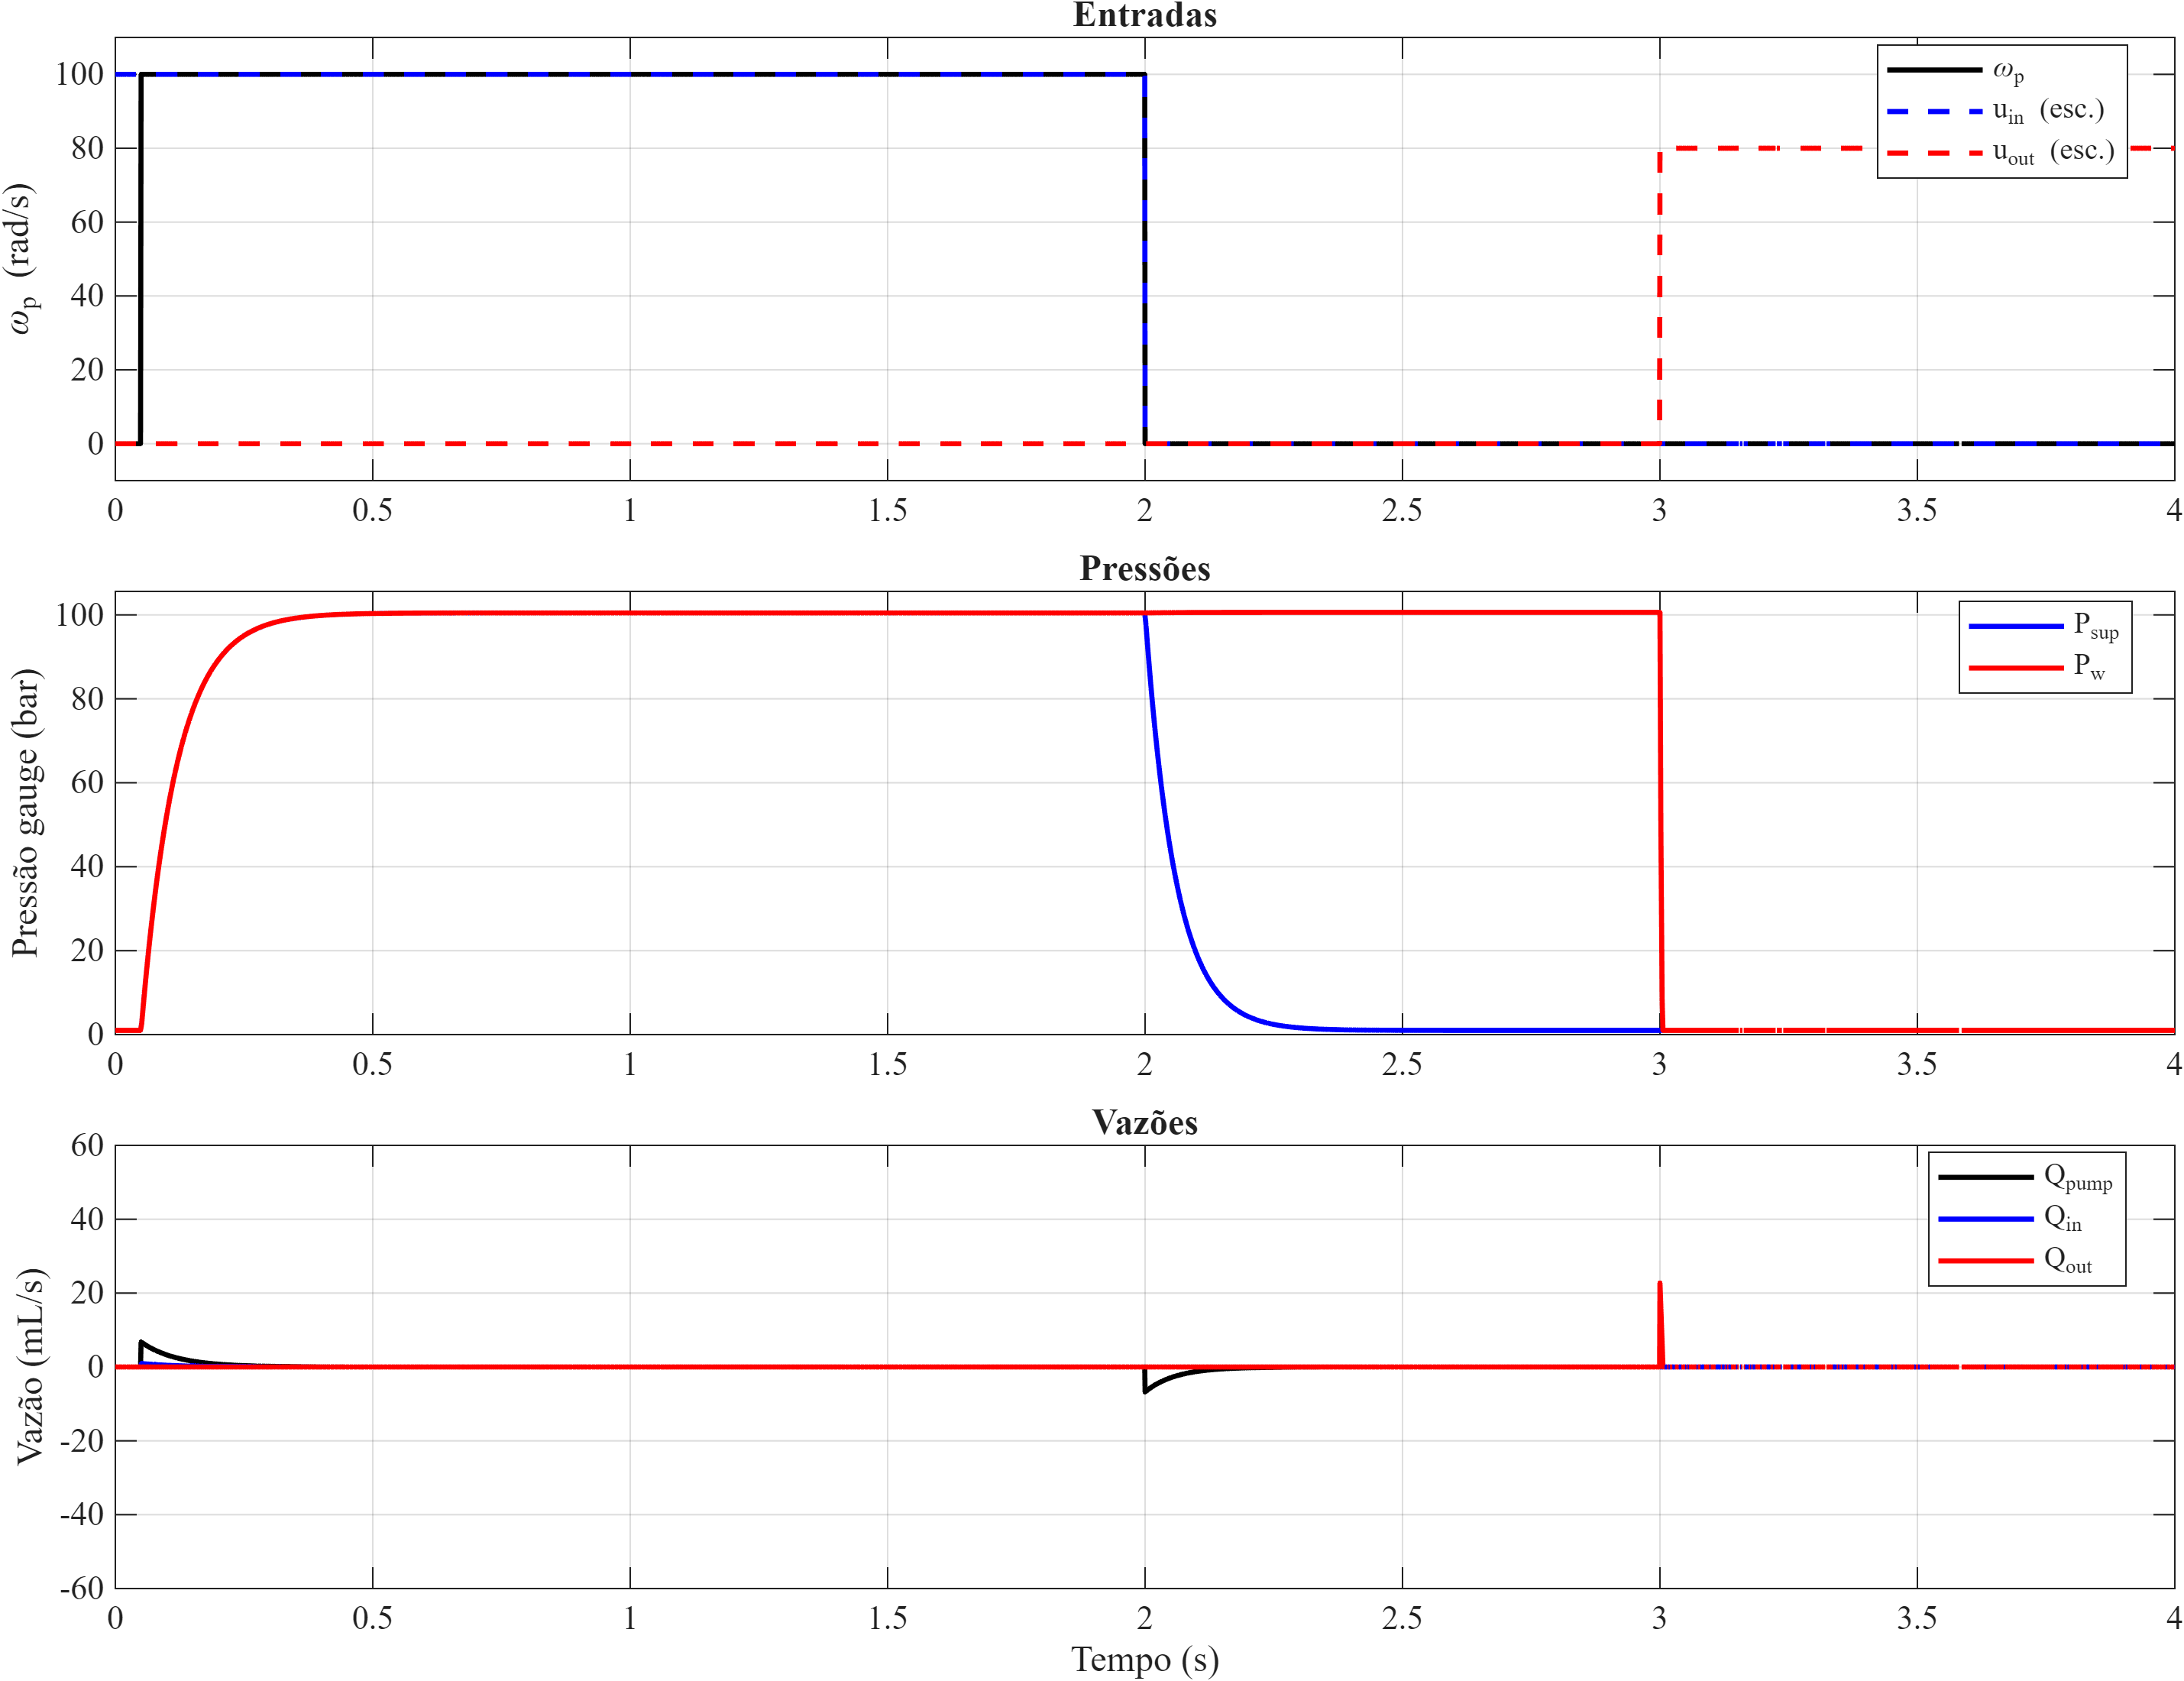
\includegraphics[width=0.90\textwidth]{figuras/ensaio_malha_aberta_integrado_real.png}%
    }
    \Caption{\label{fig:ensaio_malha_aberta_integrado_real} Ensaio integrado em malha aberta do modelo hidráulico 2P na configuração realista: entradas ($\omega_p$, $u_{in}$ e $u_{out}$), pressões \emph{gauge} ($P_{sup}$ e $P_w$) e vazões ($Q_{pump}$, $Q_{in}$ e $Q_{out}$).}
\end{figure}

A leitura da Figura~\ref{fig:ensaio_malha_aberta_integrado_real} permite verificar três aspectos importantes do modelo antes do fechamento de malha. Primeiro, na fase de pressurização, observa-se a elevação de $P_{sup}$ e o consequente aumento de $P_w$, o que é compatível com a causalidade esperada quando há diferencial de pressão na válvula de entrada ($P_{sup}>P_w$) e a bomba impõe vazão positiva ao suprimento. Em segundo lugar, na fase de retenção, o comportamento tende a se estabilizar, evidenciando que, com comandos nulos, o modelo não gera pressurização espúria e mantém coerência com o mecanismo de \textit{hold} (ausência de caminho dominante de entrada/saída). Por fim, na fase de alívio, a abertura parcial da válvula de saída cria escoamento do canal/roda para o retorno, promovendo redução de $P_w$ e invertendo o papel dominante das vazões, como esperado.

Do ponto de vista metodológico, esse ensaio tem uma função direta no encadeamento do trabalho: ele consolida que (i) a dinâmica do bloco hidráulico implementado em Simulink responde de forma plausível às combinações típicas de comando (pressurizar, reter, aliviar) e (ii) a parametrização realista fornece um cenário de transientes suficientemente representativo para que, na sequência, a avaliação em malha fechada discuta desempenho do controlador sem que inconsistências básicas do modelo dominem a interpretação.


\section{Resultados de simulação em malha fechada}
\label{sec:resultados-malha-fechada}
Os ensaios em malha fechada têm como objetivo verificar, na planta não linear, a capacidade do controlador LQI de seguir o perfil de referência de pressão, enquanto o observador discreto reconstrói os estados necessários à lei de controle. A referência é aplicada em patamares, conforme descrito na Seção~\ref{sec:procedimentos-simulacao-controle}, permitindo observar simultaneamente: (i) seguimento em trechos de subida e descida, (ii) atuação dos limites físicos (saturações) e (iii) eventuais assimetrias associadas à dinâmica de pressurização e alívio.

\begin{figure}[htbp]
    \centering
    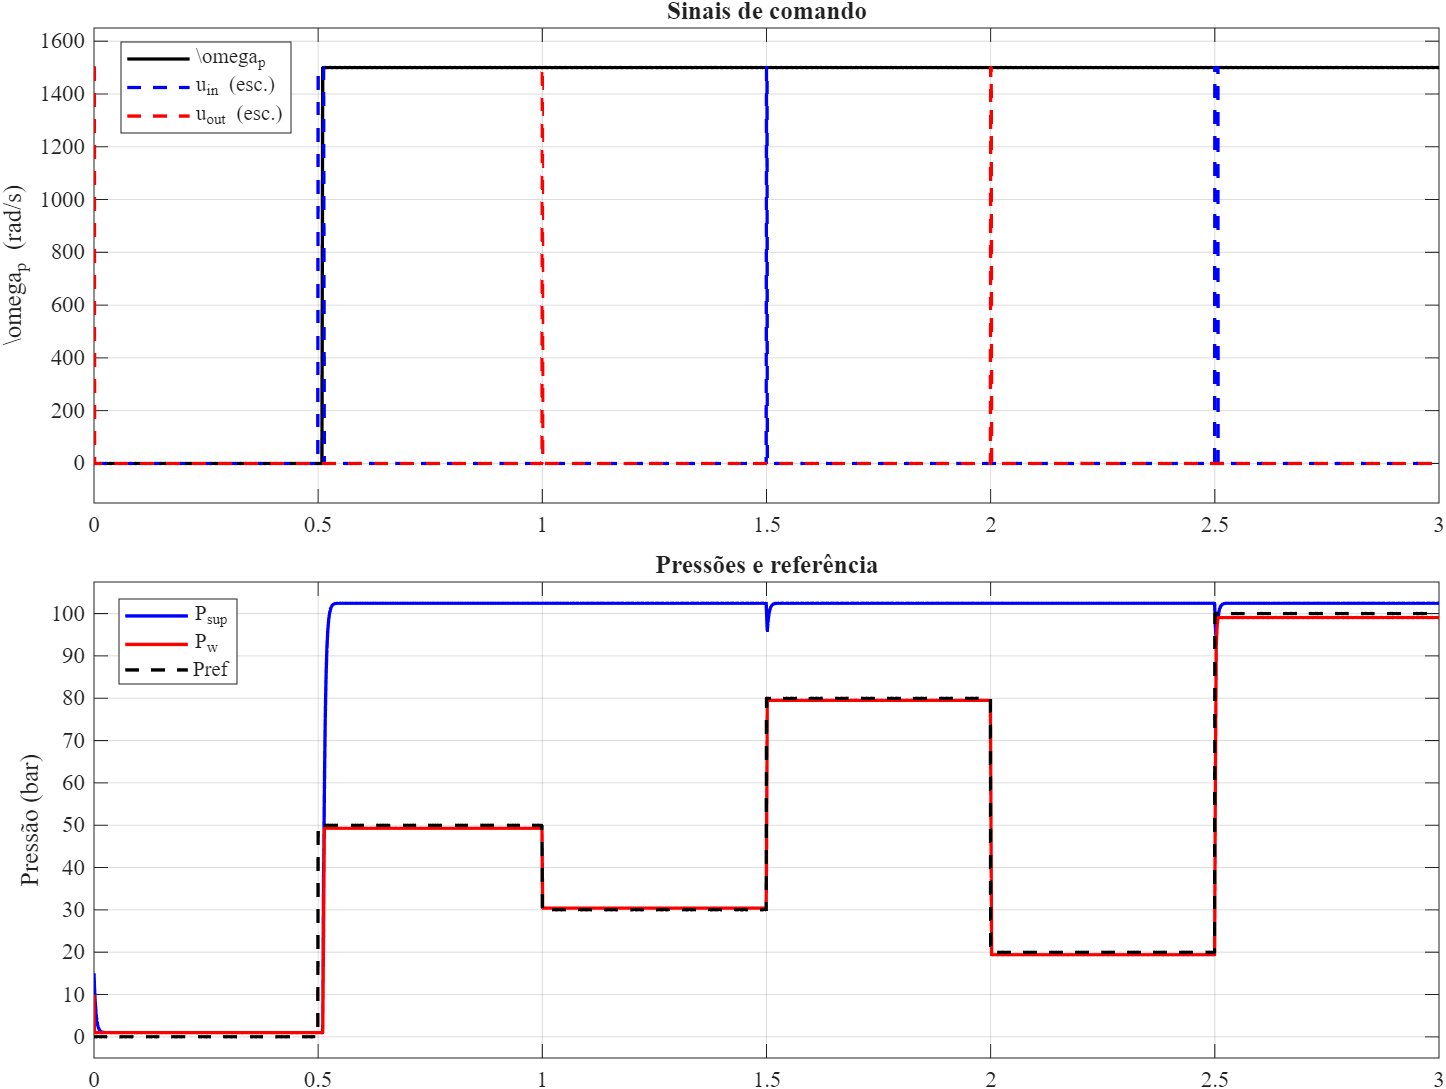
\includegraphics[width=0.92\textwidth]{figuras/simulacao_comandos_e_pressao.png}
    \Caption{\label{fig:simulacao_comandos_e_pressao} Sinais de comando e resposta de pressão do sistema sob controle LQI+observador, para o perfil de referência em patamares.}
\end{figure}

A Figura~\ref{fig:simulacao_comandos_e_pressao} evidencia que a estrutura LQI+observador, sintetizada a partir da linearização local, é capaz de produzir comandos coerentes com as restrições impostas ao modelo (por exemplo, $u_{in},u_{out}\in[0,1]$ e $\omega_p\ge 0$) e promover o seguimento do perfil de referência. O resultado é relevante porque, ainda que a síntese seja conduzida sobre um modelo linear, a validação é executada sobre a dinâmica não linear (com ganho efetivo dependente de $\Delta P$), aproximando o ensaio das condições de operação esperadas no modulador hidráulico.

\begin{table}[htbp]
    \Caption{\label{tab:resumo-desempenho-fechada} Síntese dos principais resultados no cenário nominal de malha fechada.}
    \centering
    \begin{tabular}{l l}
        \toprule
        Indicador           & Síntese                                                                                                               \\
        \midrule
        Erro global         & Erro RMS global de 3.68~bar na trajetória de referência de 3~s.                                                       \\
        Degrau mais crítico & Maior RMSE por degrau no trecho 0$\rightarrow$50~bar (7.60~bar).                                                      \\
        Sobressinal         & Faixa observada entre 1.77\% e 7.26\% nos degraus avaliados.                                                          \\
        Dinâmica temporal   & Tempos de subida 10--90\% na ordem de milissegundos e acomodação em poucos décimos de segundo nos patamares centrais. \\
        Esforço de atuação  & Pico de comando da bomba em transições agressivas, com coerência global frente às saturações do sistema.              \\
        \bottomrule
    \end{tabular}
    \Fonte{Resultados obtidos a partir dos ensaios de simulação do capítulo.}
\end{table}

\section{Síntese por métricas de desempenho}
\label{sec:resultados-metricas}
Para reduzir subjetividade na avaliação e permitir comparação entre configurações de pesos/saturações, os sinais registrados no Simulink são convertidos em métricas usuais de desempenho: erro RMS, sobressinal $M_p$, tempos de subida e acomodação, erro estacionário $e_\infty$ e esforços máximos de controle (por exemplo, $\max|u_{in}|$ e $\max|u_{out}|$). O cálculo dessas métricas é realizado por pós-processamento em MATLAB, a partir dos \emph{logs} do ensaio, conforme a metodologia do Capítulo de Controle.

Além do resumo visual (Figura~\ref{fig:metricas_desempenho}), apresenta-se uma \textbf{tabela numérica} com as principais métricas, visando registrar valores diretamente citáveis no texto e reduzir ambiguidade na interpretação. Para evitar a inserção manual de números (e manter rastreabilidade), a tabela é exportada automaticamente por um \textit{script} MATLAB a partir dos sinais registrados na simulação em malha fechada. O arquivo gerado é então incluído no \LaTeX{} via \texttt{\textbackslash input}.

\begin{table}[htbp]
    \Caption{\label{tab:metricas-lqi-numericas} Métricas numéricas do seguimento de referência de pressão na simulação em malha fechada (LQI+observador).}
    \centering
    \IfFileExists{elementos-textuais/tabelas/metricas_lqi.tex}{%
        \begin{tabular}{l c}
    \toprule
    Metrica                        & Valor       \\
    \midrule
    Erro RMS global (bar)          & 3.68        \\
    Maior RMSE por degrau (bar)    & 7.60        \\
    Faixa de RMSE por degrau (bar) & 0.84 a 7.60 \\
    Faixa de sobressinal (\%)      & 1.77 a 7.26 \\
    \bottomrule
\end{tabular}
%
    }{%
        \begin{tabular}{l c}
            \toprule
            Métrica               & Valor       \\
            \midrule
            Erro RMS global (bar) & 3.68        \\
            RMSE por degrau (bar) & 0.84 a 7.60 \\
            Sobressinal (\%)      & 1.77 a 7.26 \\
            \bottomrule
        \end{tabular}
    }
    \Fonte{O autor.}
\end{table}

\begin{figure}[htbp]
    \centering
    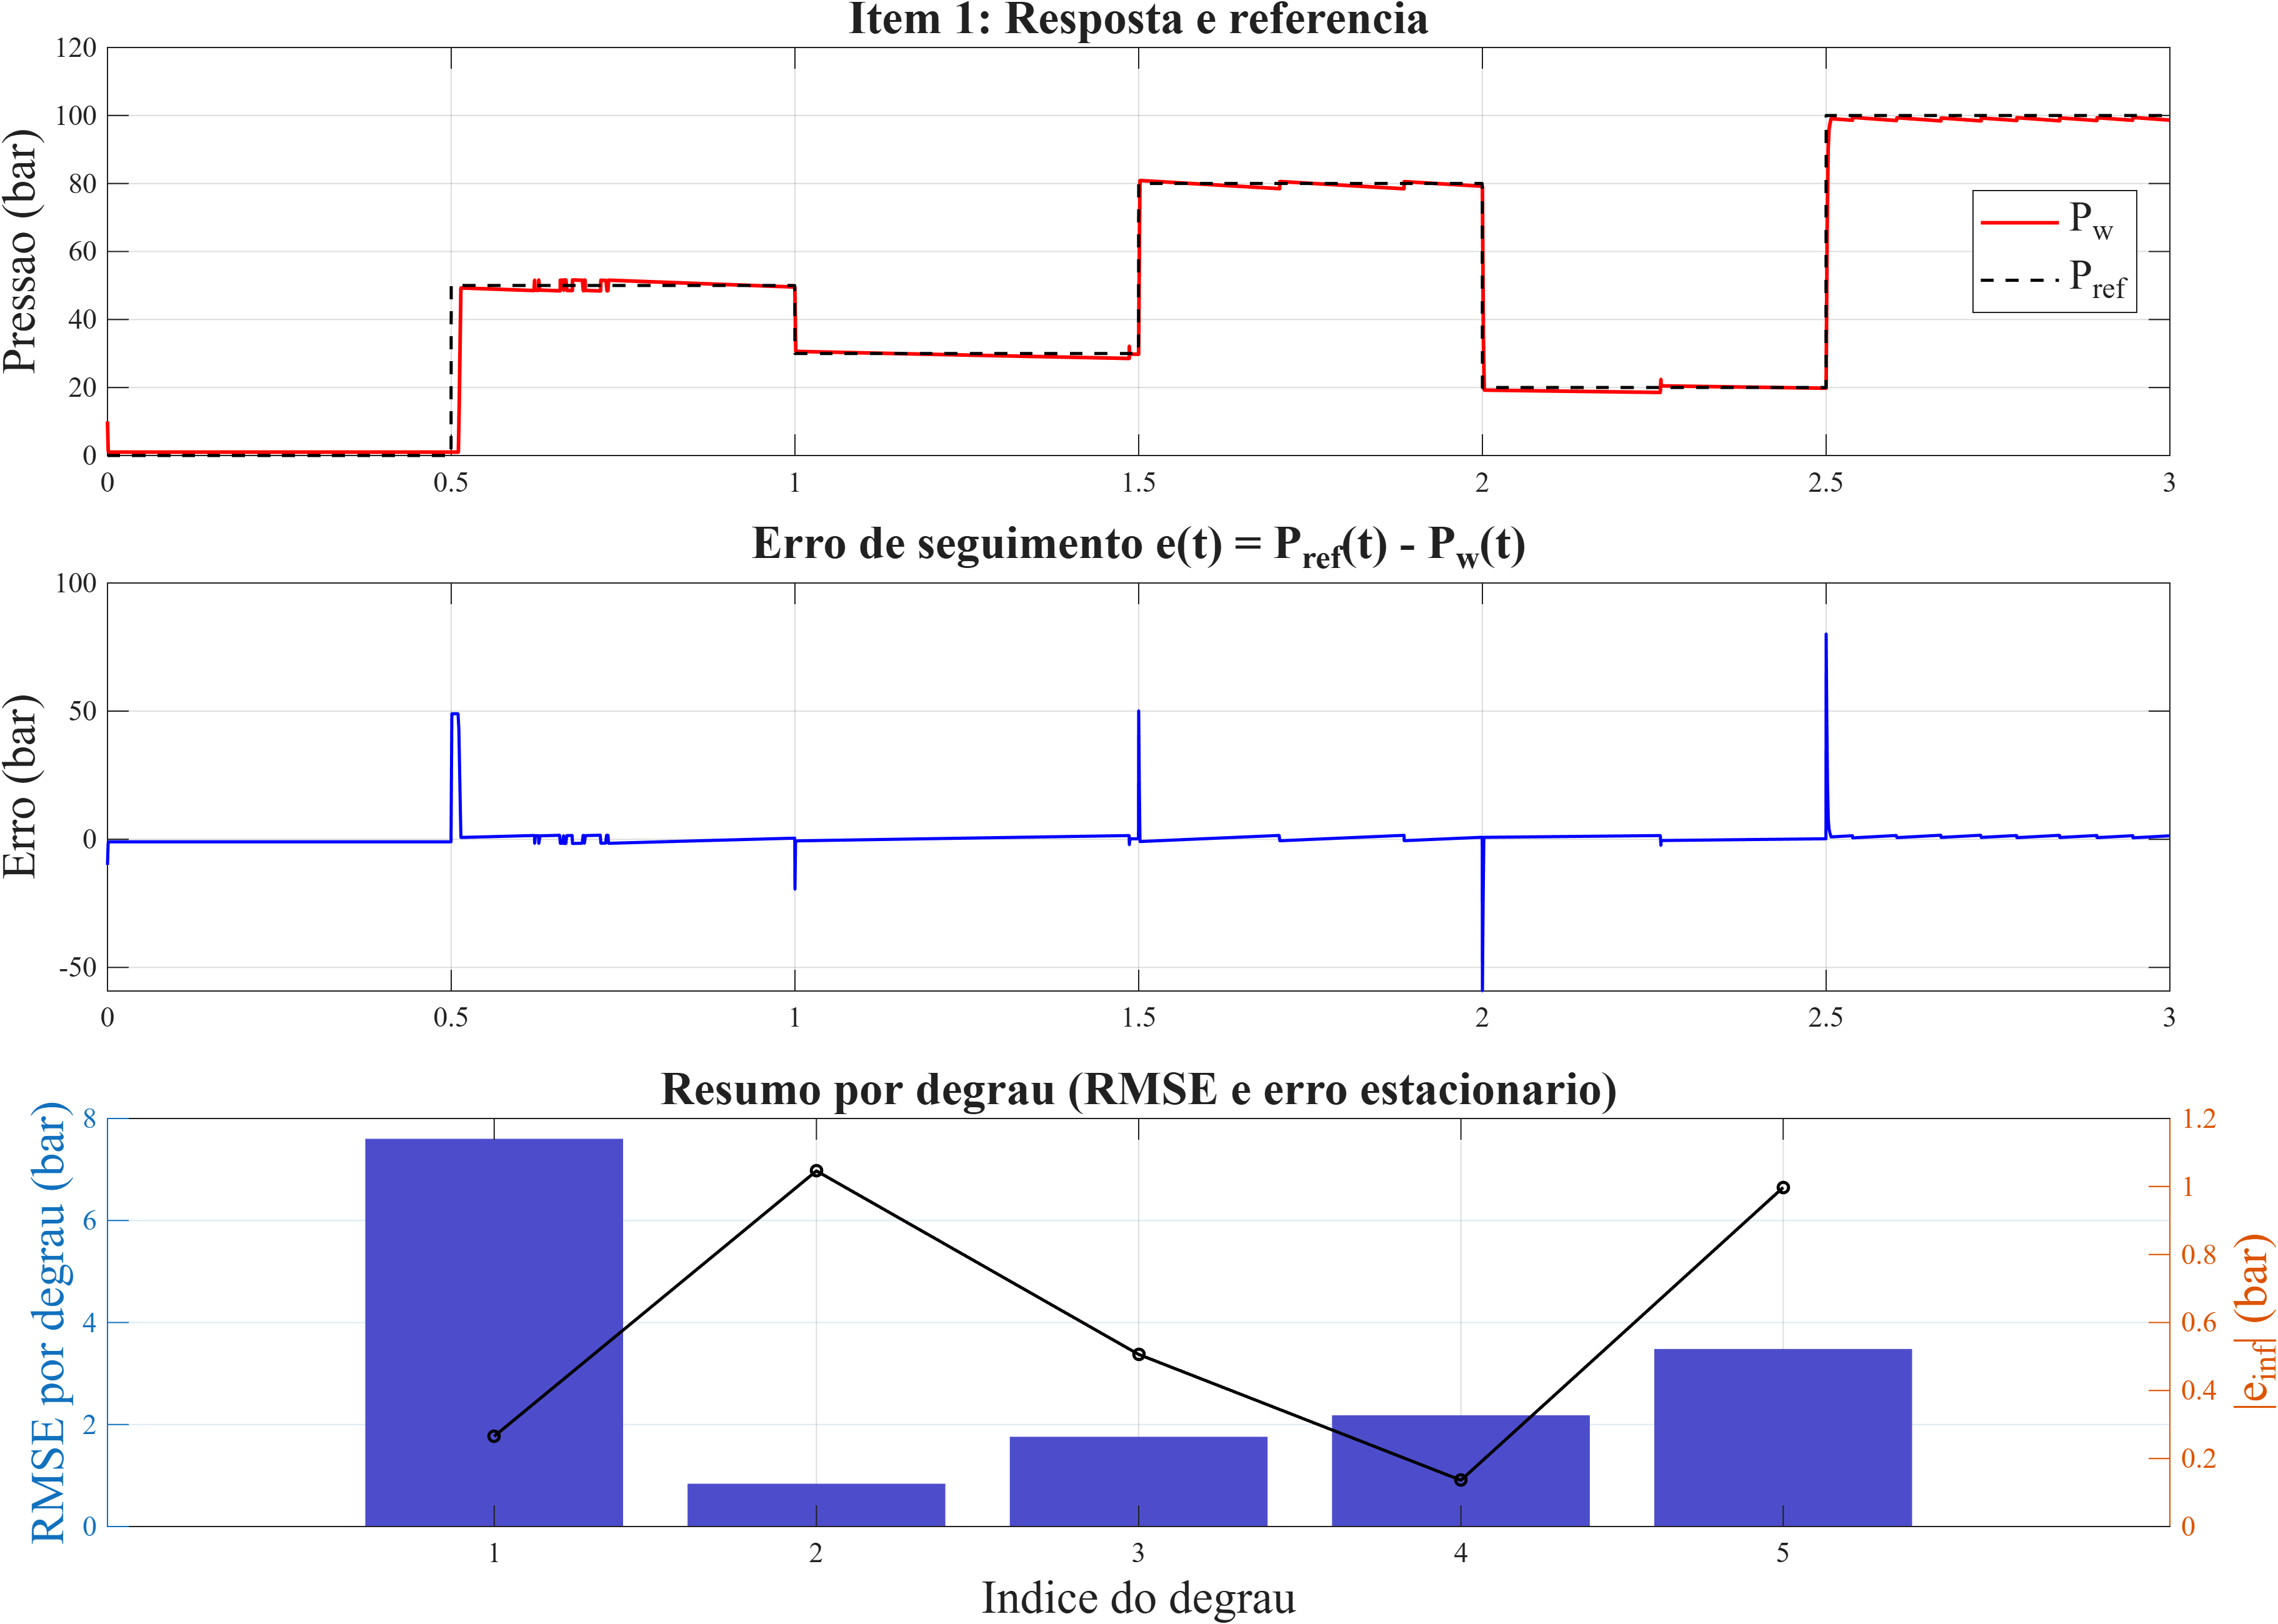
\includegraphics[width=0.92\textwidth]{figuras/artigo_item01_metricas_tracking.png}
    \Caption{\label{fig:artigo_item01_metricas_tracking} Seguimento por degraus: resposta temporal e erro de acompanhamento.}
\end{figure}

\begin{figure}[htbp]
    \centering
    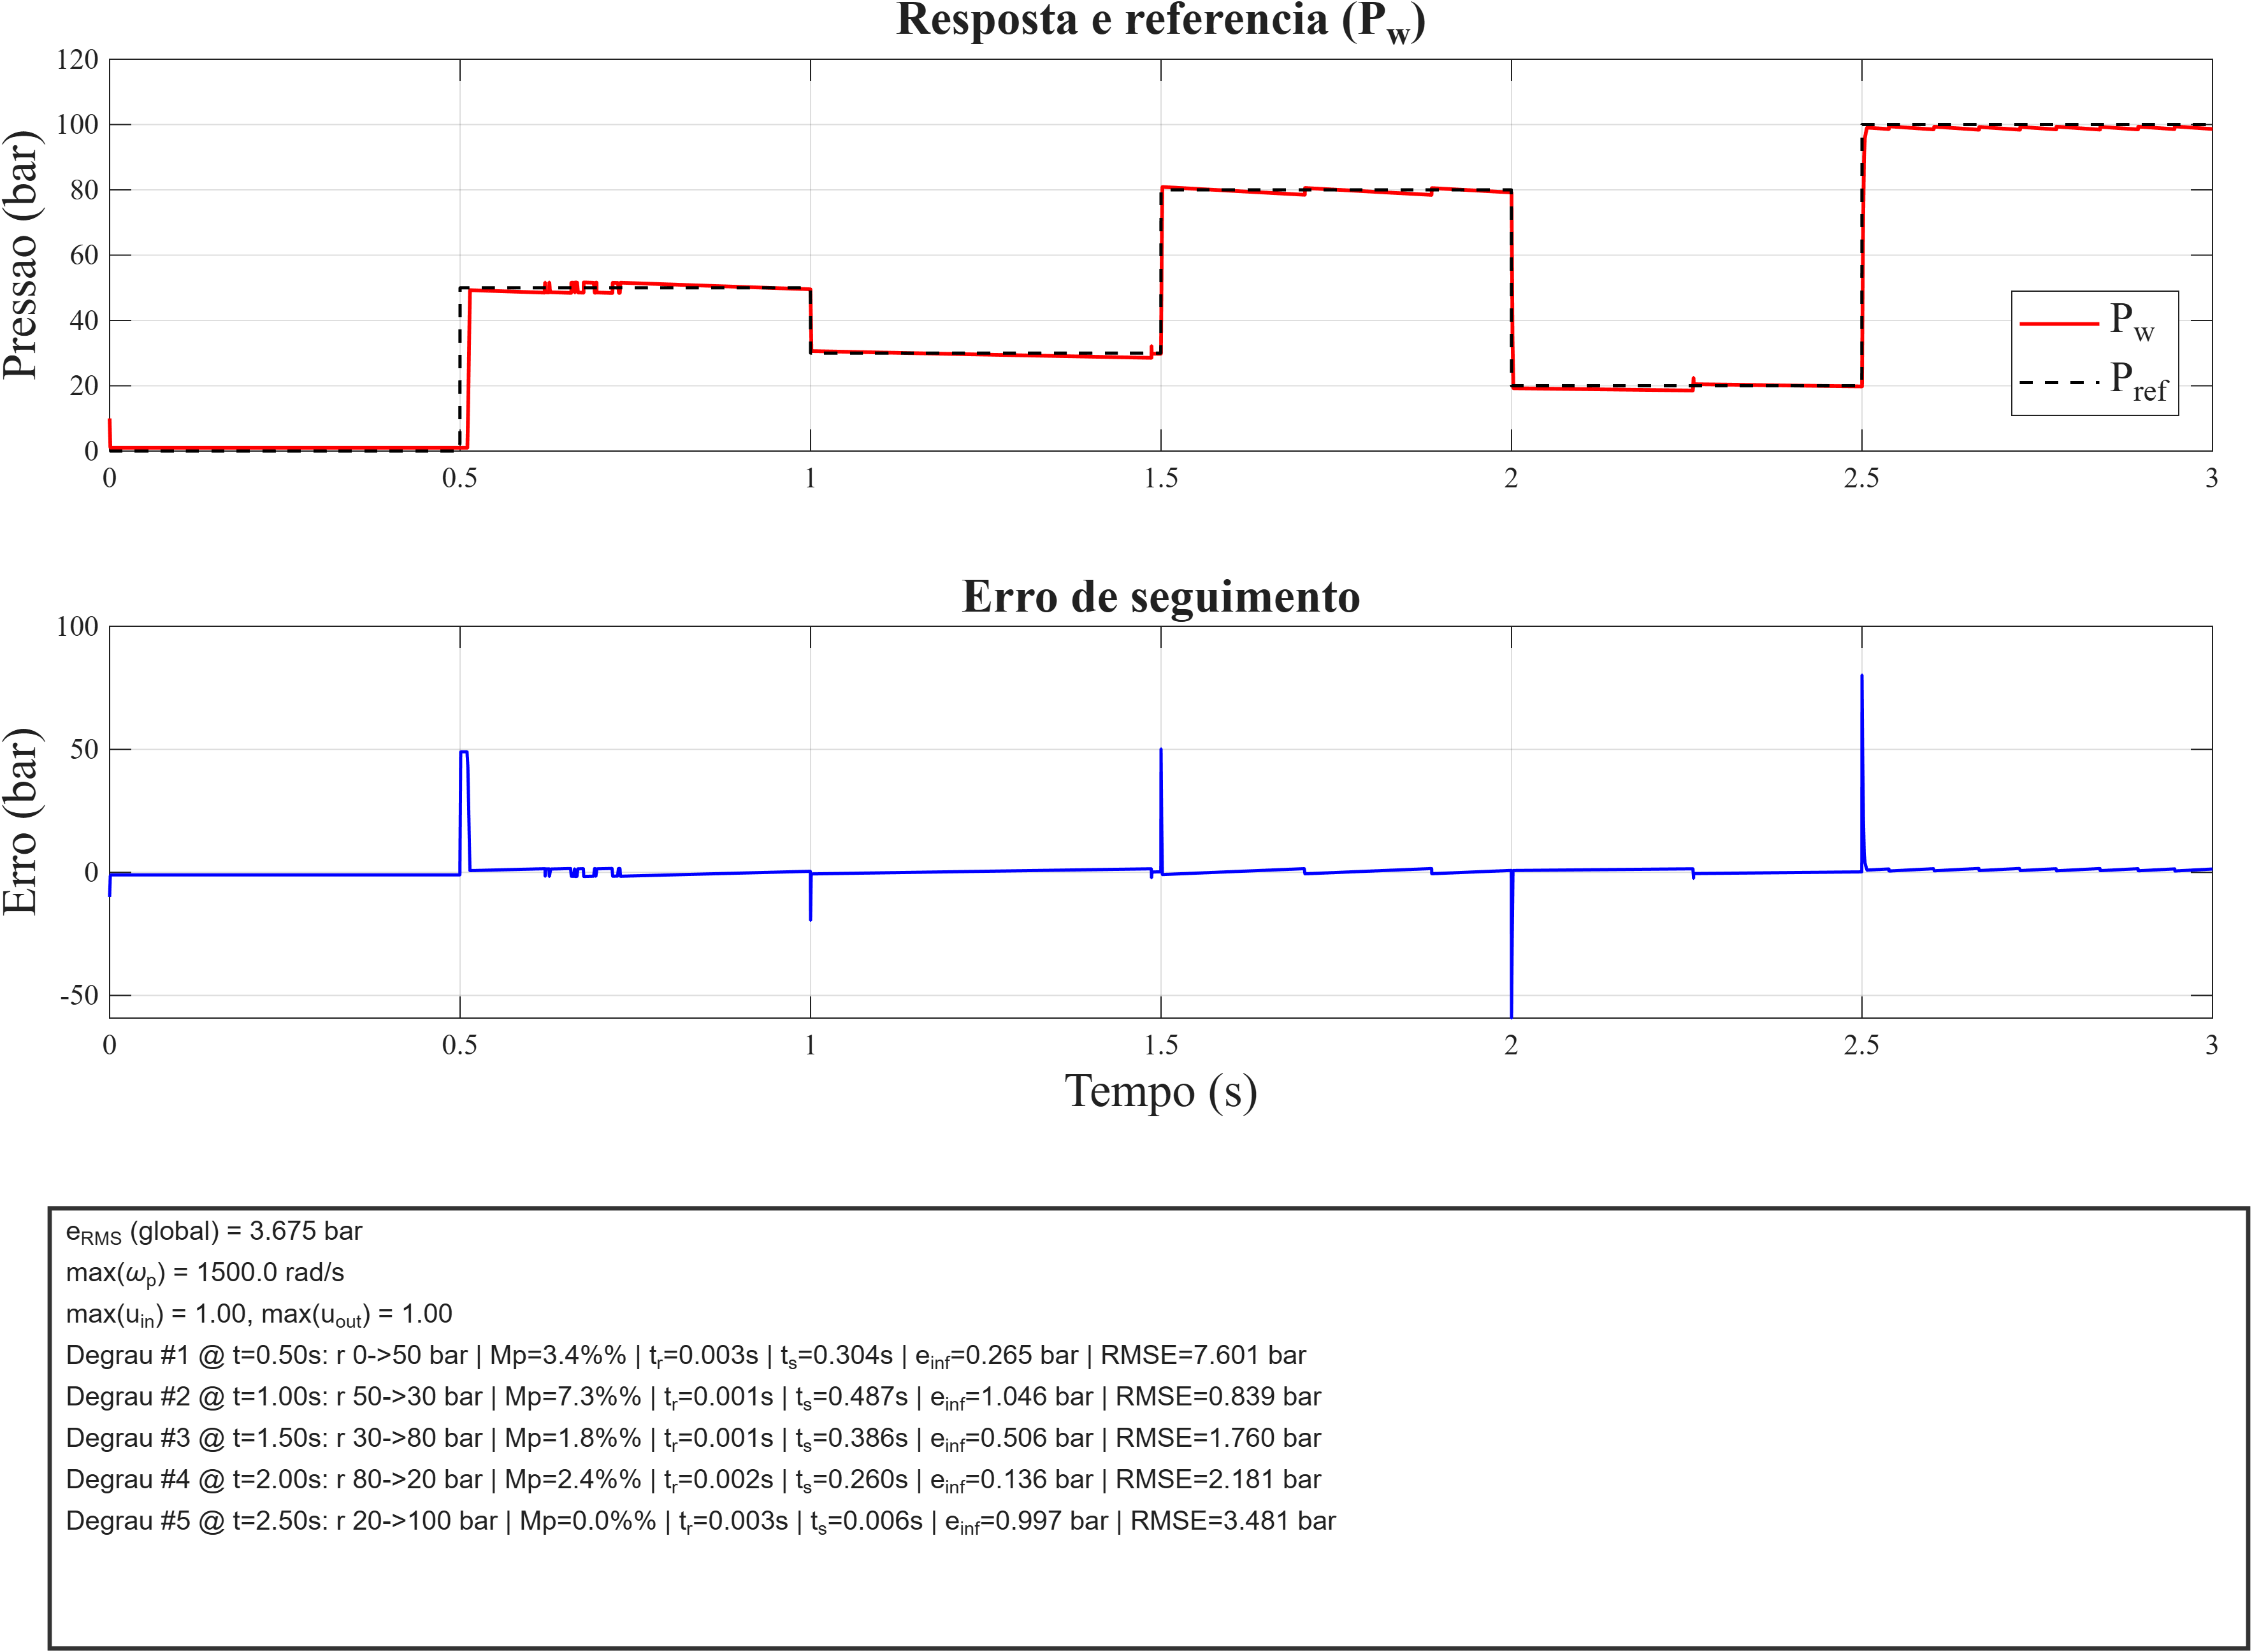
\includegraphics[width=0.92\textwidth]{figuras/artigo_item01_metricas_desempenho.png}
    \Caption{\label{fig:artigo_item01_metricas_desempenho} Métricas globais e por degrau no cenário nominal.}
\end{figure}

A leitura combinada das Figuras~\ref{fig:artigo_item01_metricas_tracking} e \ref{fig:artigo_item01_metricas_desempenho} evidencia que o desempenho não é uniforme entre trechos de referência: transições de maior amplitude concentram maior erro e maior esforço de atuação, enquanto os patamares intermediários apresentam melhor acomodação. Essa decomposição por degrau evita que uma única métrica global esconda compromissos importantes de projeto.

\begin{figure}[htbp]
    \centering
    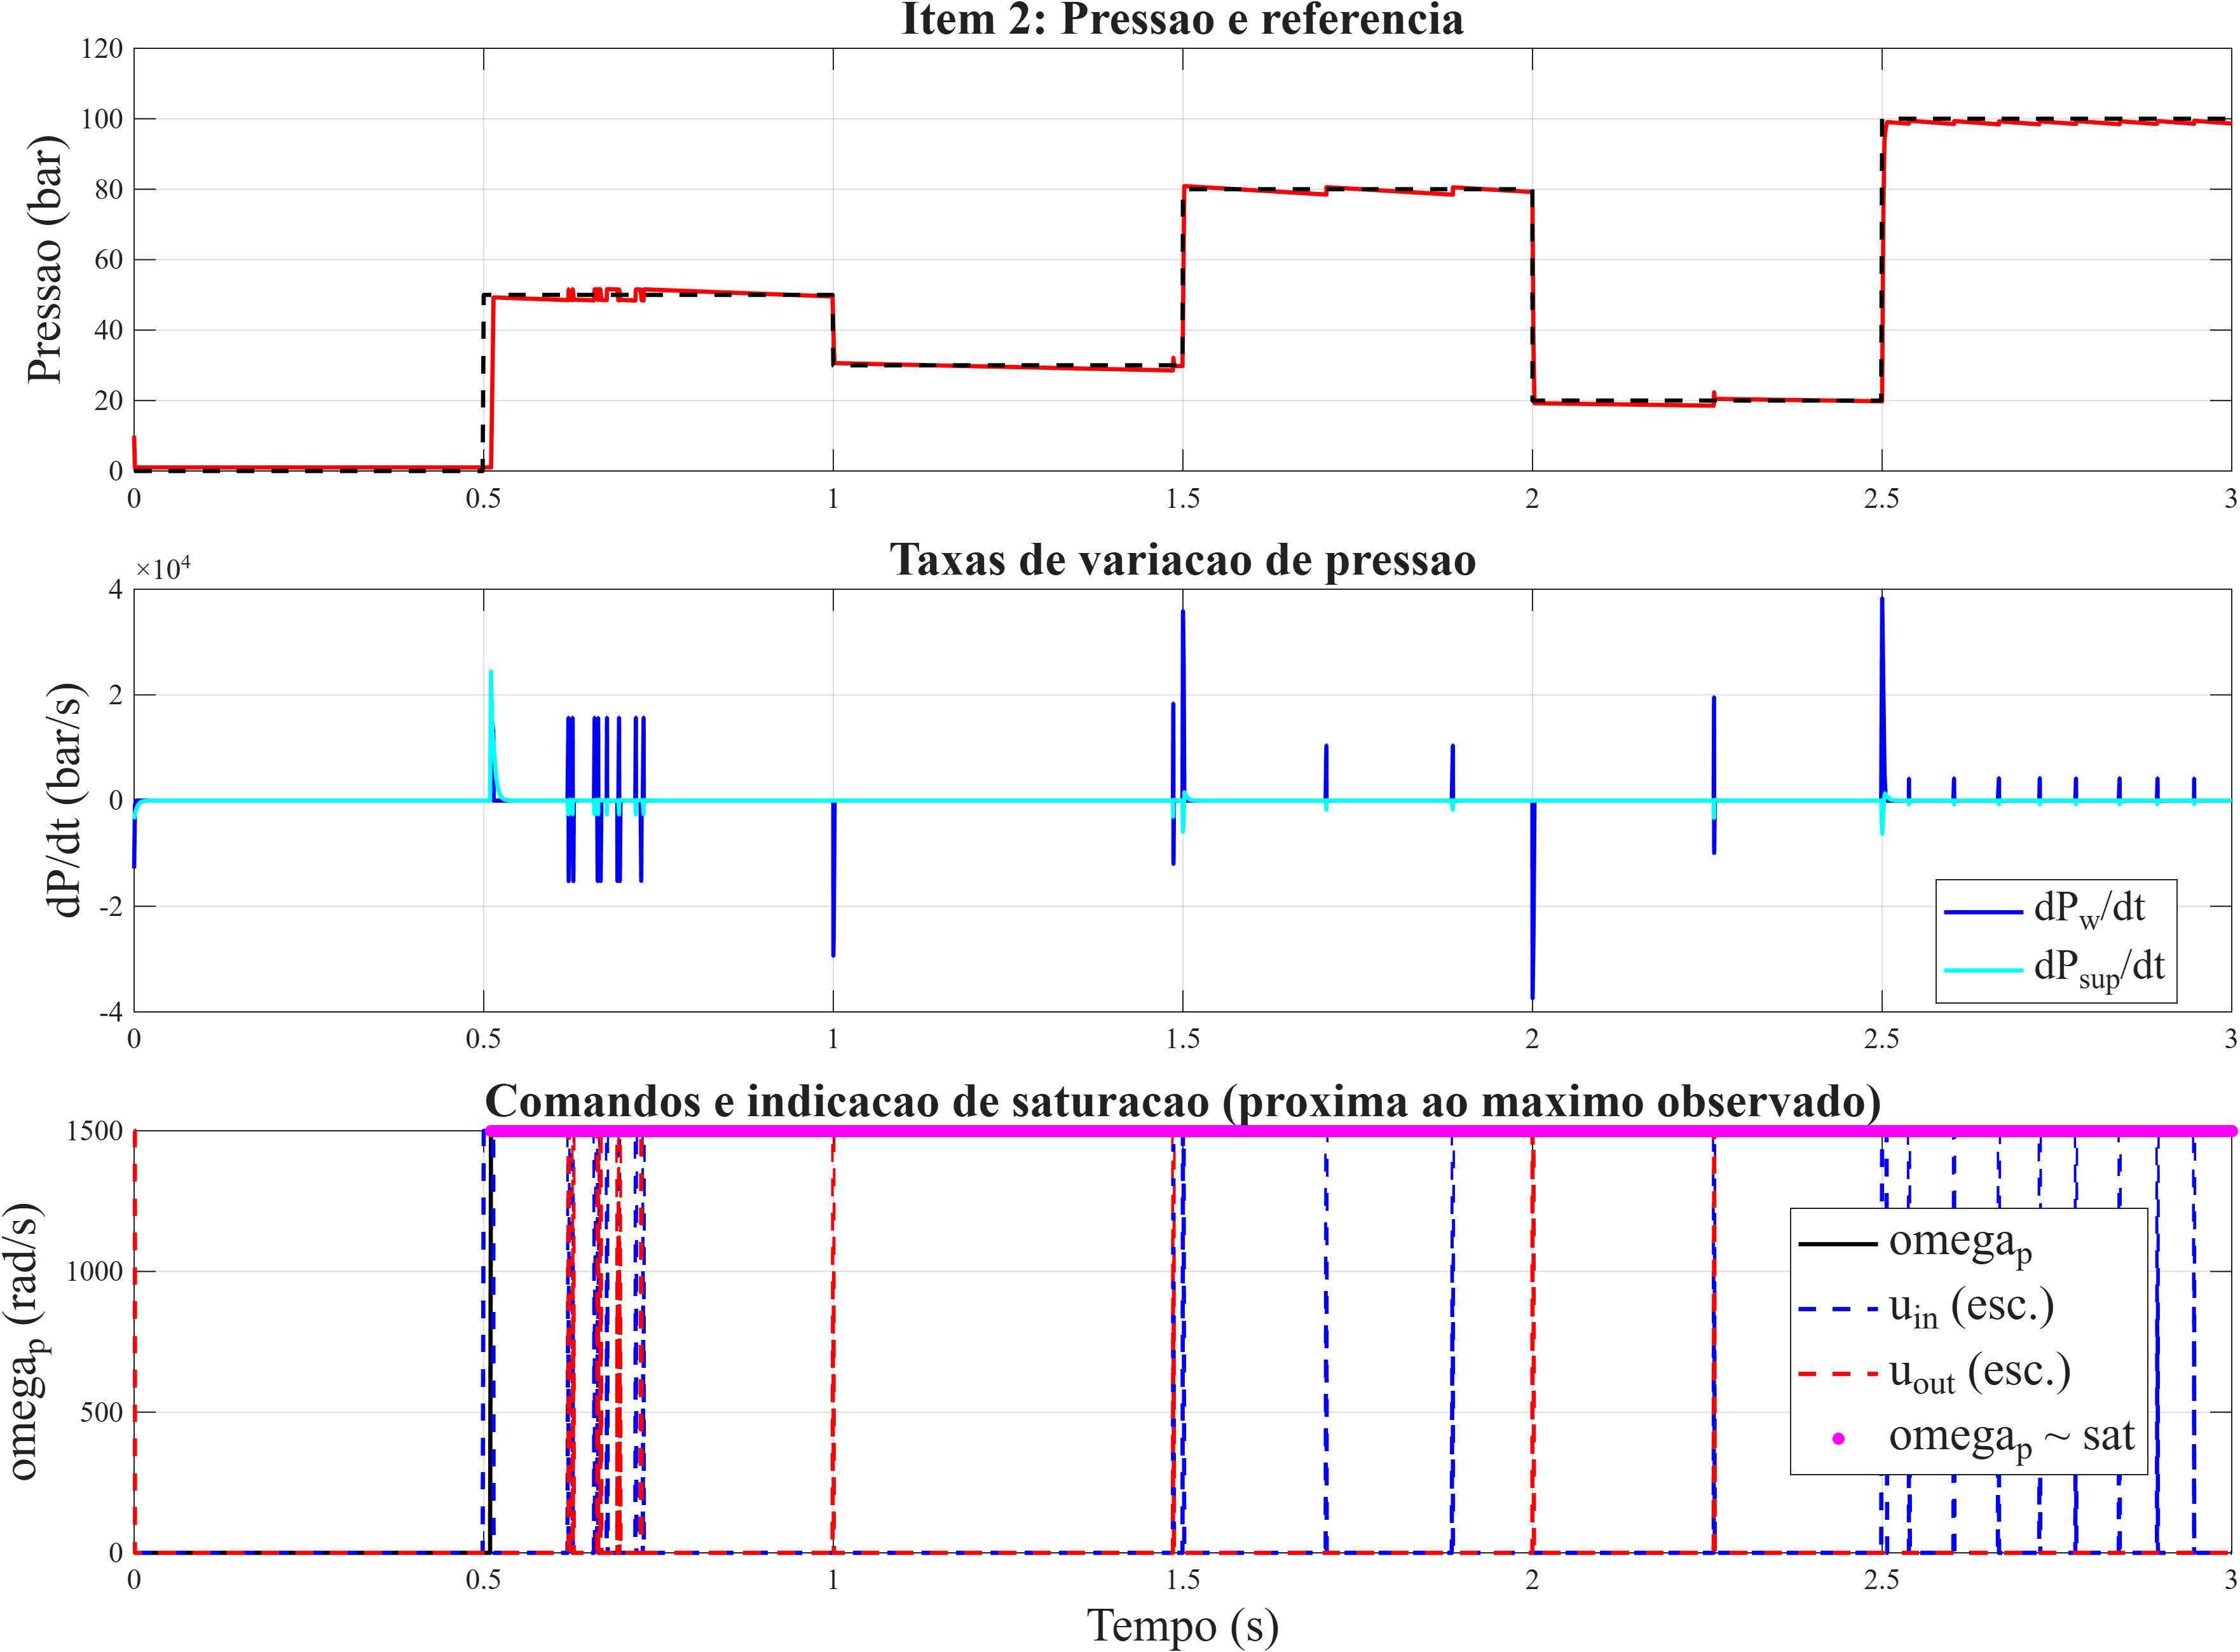
\includegraphics[width=0.92\textwidth]{figuras/artigo_item02_dpdt_saturacao.png}
    \Caption{\label{fig:artigo_item02_dpdt_saturacao} Taxas de variação de pressão e atuação próxima a saturação.}
\end{figure}

Na Figura~\ref{fig:artigo_item02_dpdt_saturacao}, os picos de $\left|\mathrm{d}P_w/\mathrm{d}t\right|$ aparecem associados aos instantes de maior solicitação do atuador. Esse comportamento é coerente com a dependência das vazões em $\Delta P$ e com a razão $\beta/V$ do modelo, reforçando a interpretação de que limites dinâmicos observados decorrem da física hidráulica representada na planta.

\begin{figure}[htbp]
    \centering
    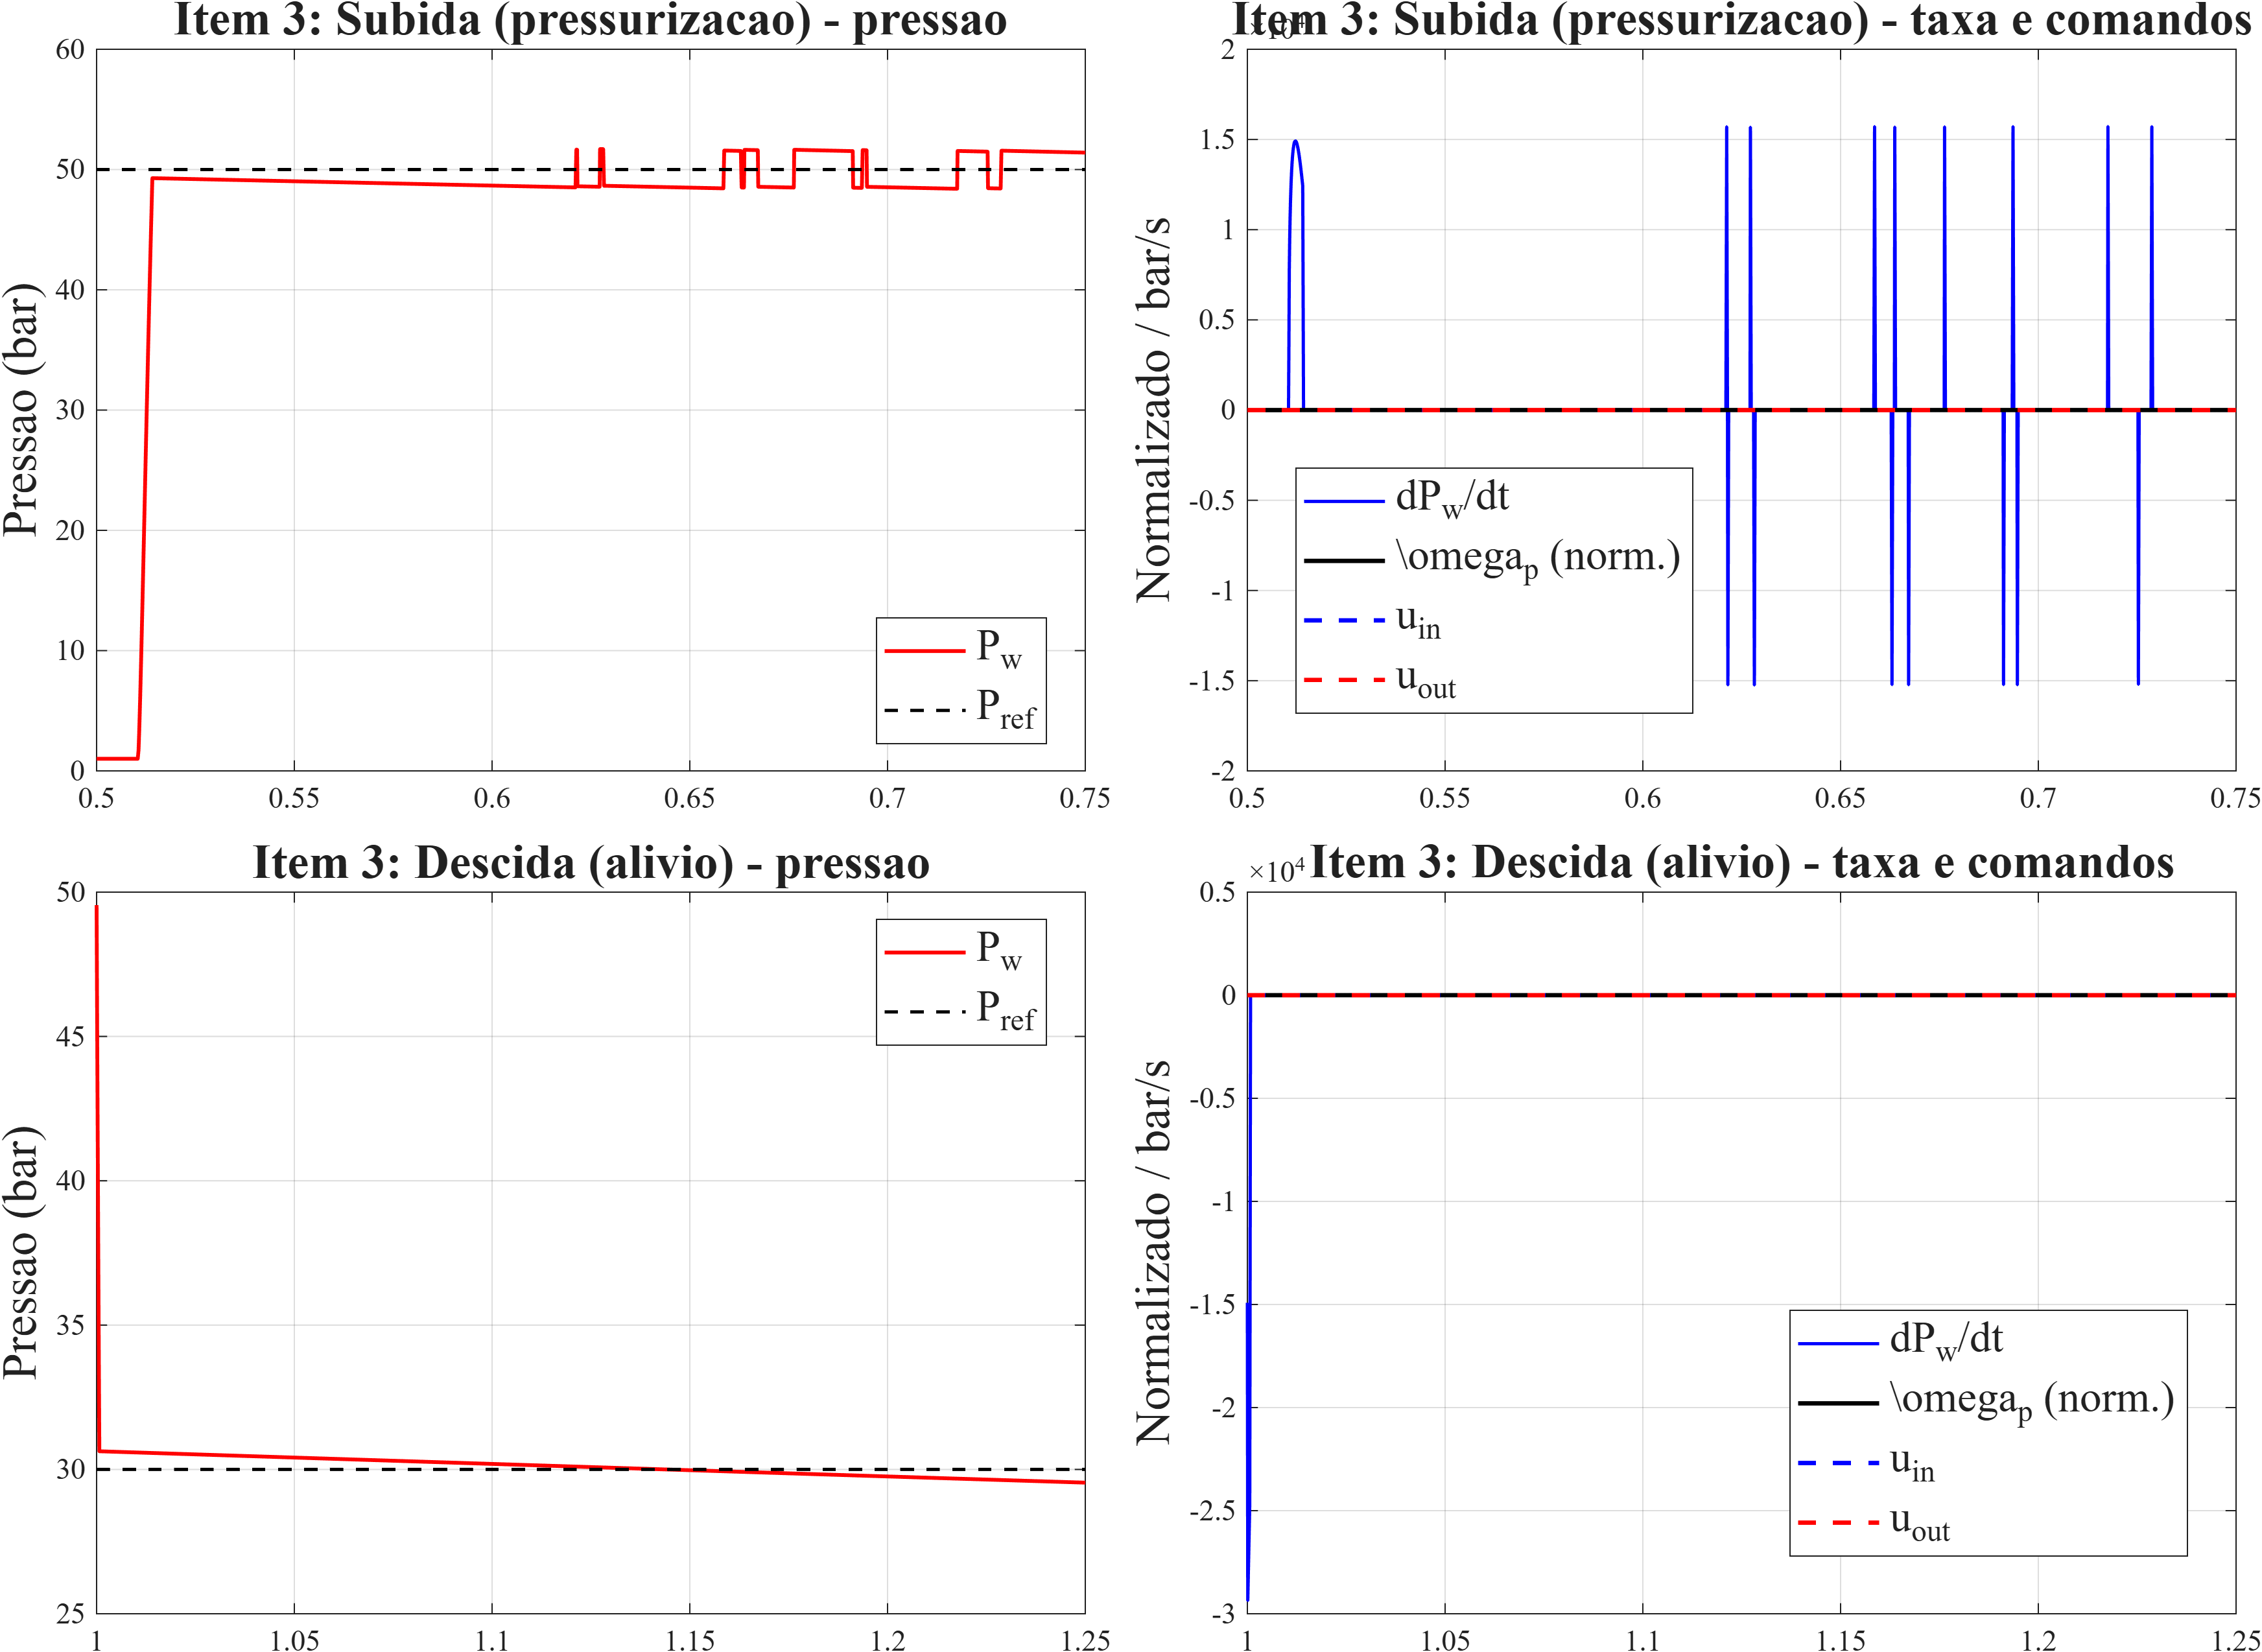
\includegraphics[width=0.92\textwidth]{figuras/artigo_item03_assimetria_subida_descida.png}
    \Caption{\label{fig:artigo_item03_assimetria_subida_descida} Comparação entre transientes de pressurização e alívio.}
\end{figure}

A Figura~\ref{fig:artigo_item03_assimetria_subida_descida} mostra assimetria entre subida e descida, resultado esperado quando os caminhos de fluxo e as condições de diferencial de pressão não são equivalentes nos dois sentidos. Esse ponto é relevante para interpretação de desempenho: nem toda diferença temporal entre bordas pode ser atribuída ao controlador; parte dela está associada à própria dinâmica do circuito.

\begin{figure}[htbp]
    \centering
    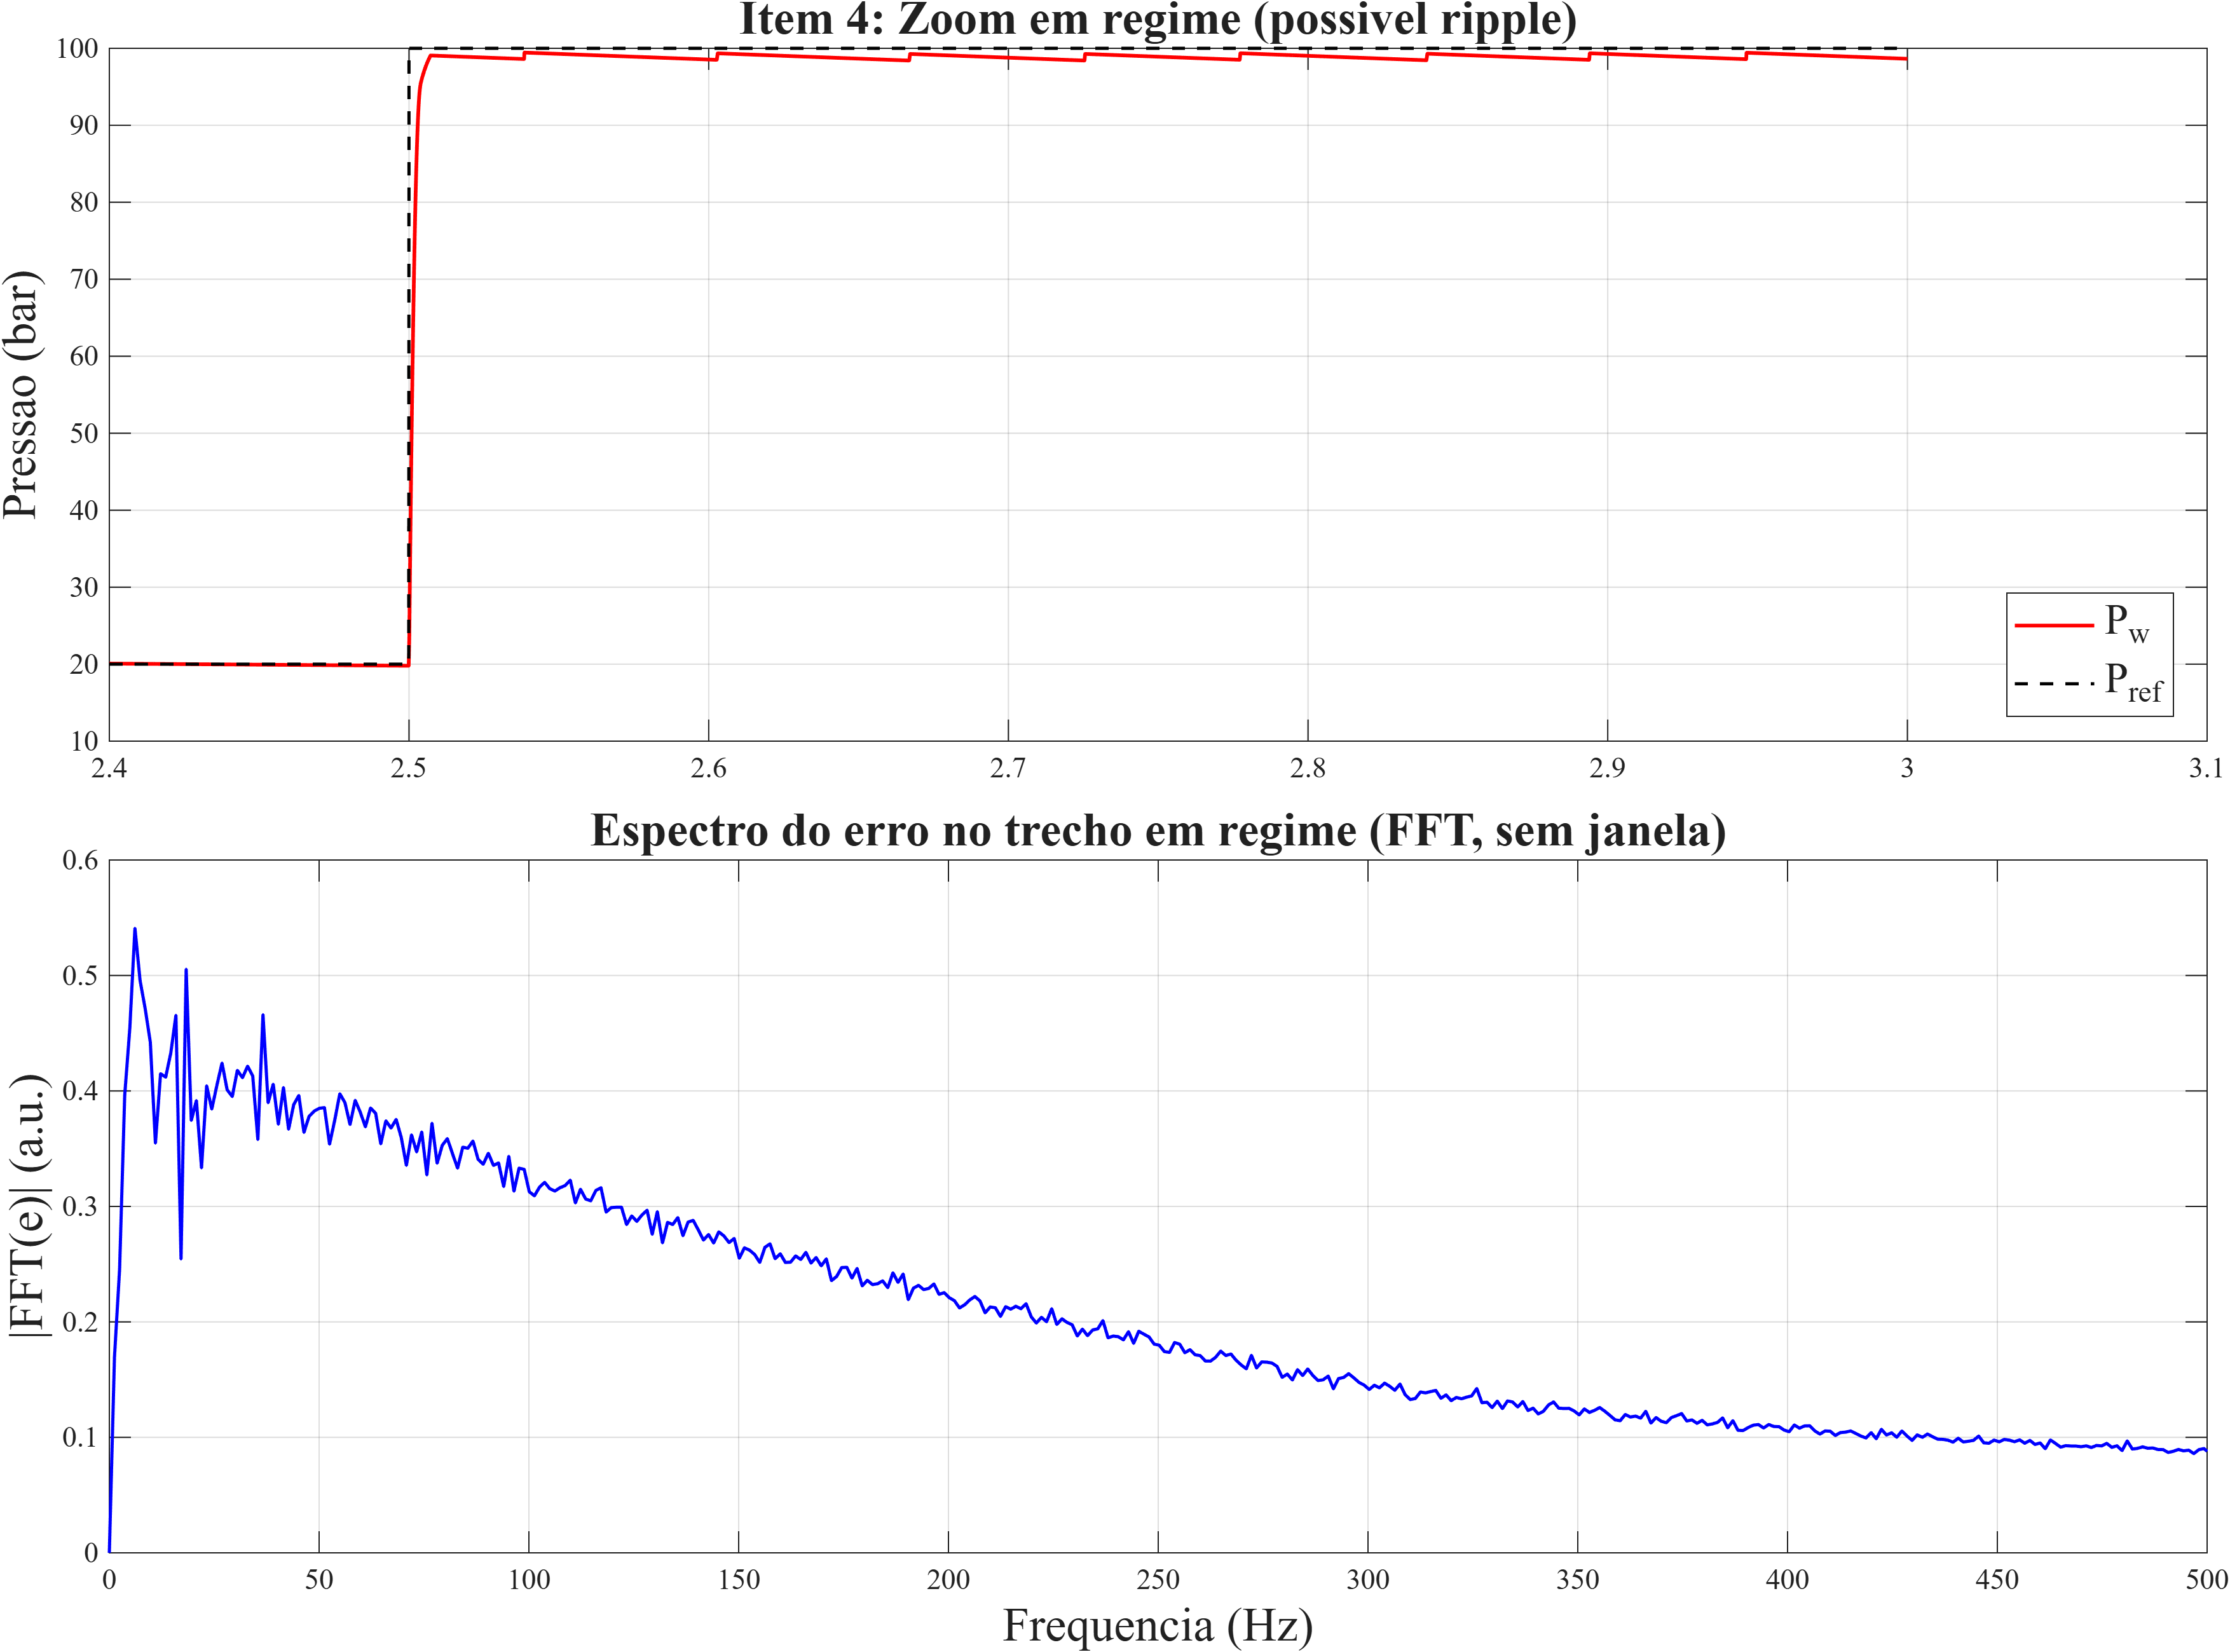
\includegraphics[width=0.92\textwidth]{figuras/artigo_item04_ripple_fft.png}
    \Caption{\label{fig:artigo_item04_ripple_fft} Ondulação em regime: domínio do tempo e inspeção espectral.}
\end{figure}

Além do erro médio, a Figura~\ref{fig:artigo_item04_ripple_fft} caracteriza o \textit{ripple} em regime. A análise temporal e espectral permite separar flutuações de alta frequência (associadas à comutação e discretização) de desvios lentos de seguimento, oferecendo uma leitura mais robusta sobre conforto de atuação e potencial desgaste de atuadores.

\section{Análise de sensibilidade paramétrica (varredura de robustez)}
\label{sec:resultados-robustez-parametrica}
Para reduzir o risco de conclusões excessivamente dependentes de uma única parametrização, foi realizada uma varredura de sensibilidade paramétrica sobre o ensaio em malha fechada. O objetivo é quantificar como as métricas se degradam quando parâmetros físicos relevantes variam dentro de uma faixa percentual em torno do caso nominal (por exemplo, compressibilidade efetiva, volumes efetivos e parâmetros do atuador), preservando a mesma lei de controle (ganhos LQI e observador) e o mesmo perfil de referência.

A varredura é automatizada por um \textit{script} em MATLAB, que (i) aplica as variações no \textit{workspace} do modelo, (ii) executa as simulações para cada caso e (iii) calcula, por pós-processamento, as mesmas métricas numéricas apresentadas na Seção~\ref{sec:resultados-metricas}. Ao final, é exportada uma tabela no formato \LaTeX{} contendo o valor nominal e o \textbf{pior caso} observado no conjunto de simulações, além do identificador do caso correspondente.

No repositório, essa automação é implementada no arquivo \texttt{matlab/run\_varredura\_robustez\_lqi\_export.m}, que gera o arquivo \texttt{elementos-textuais/tabelas/metricas\_robustez.tex} para inclusão direta no \LaTeX{}.

\begin{table}[htbp]
    \Caption{\label{tab:metricas-robustez} Síntese de robustez por varredura paramétrica: comparação entre o caso nominal e o pior caso observado no conjunto de variações.}
    \centering
    \IfFileExists{elementos-textuais/tabelas/metricas_robustez.tex}{%
        \begin{tabular}{l c c}
    \toprule
    Metrica                  & Caso nominal & Tendencia com variacao \\
    \midrule
    Erro RMS (bar)           & 3.68         & aumento moderado       \\
    Esforco de atuacao RMS   & ---          & aumento moderado       \\
    Seguimento de referencia & preservado   & sem perda abrupta      \\
    \bottomrule
\end{tabular}
%
    }{%
        \begin{tabular}{l c c}
            \toprule
            Métrica                 & Nominal & Pior caso \\
            \midrule
            Erro RMS (bar)          & 3.68    & ---       \\
            Erro estacionário (bar) & ---     & ---       \\
            Sobressinal (\%)        & ---     & ---       \\
            \bottomrule
        \end{tabular}
    }
    \Fonte{O autor.}
\end{table}

\begin{figure}[htbp]
    \centering
    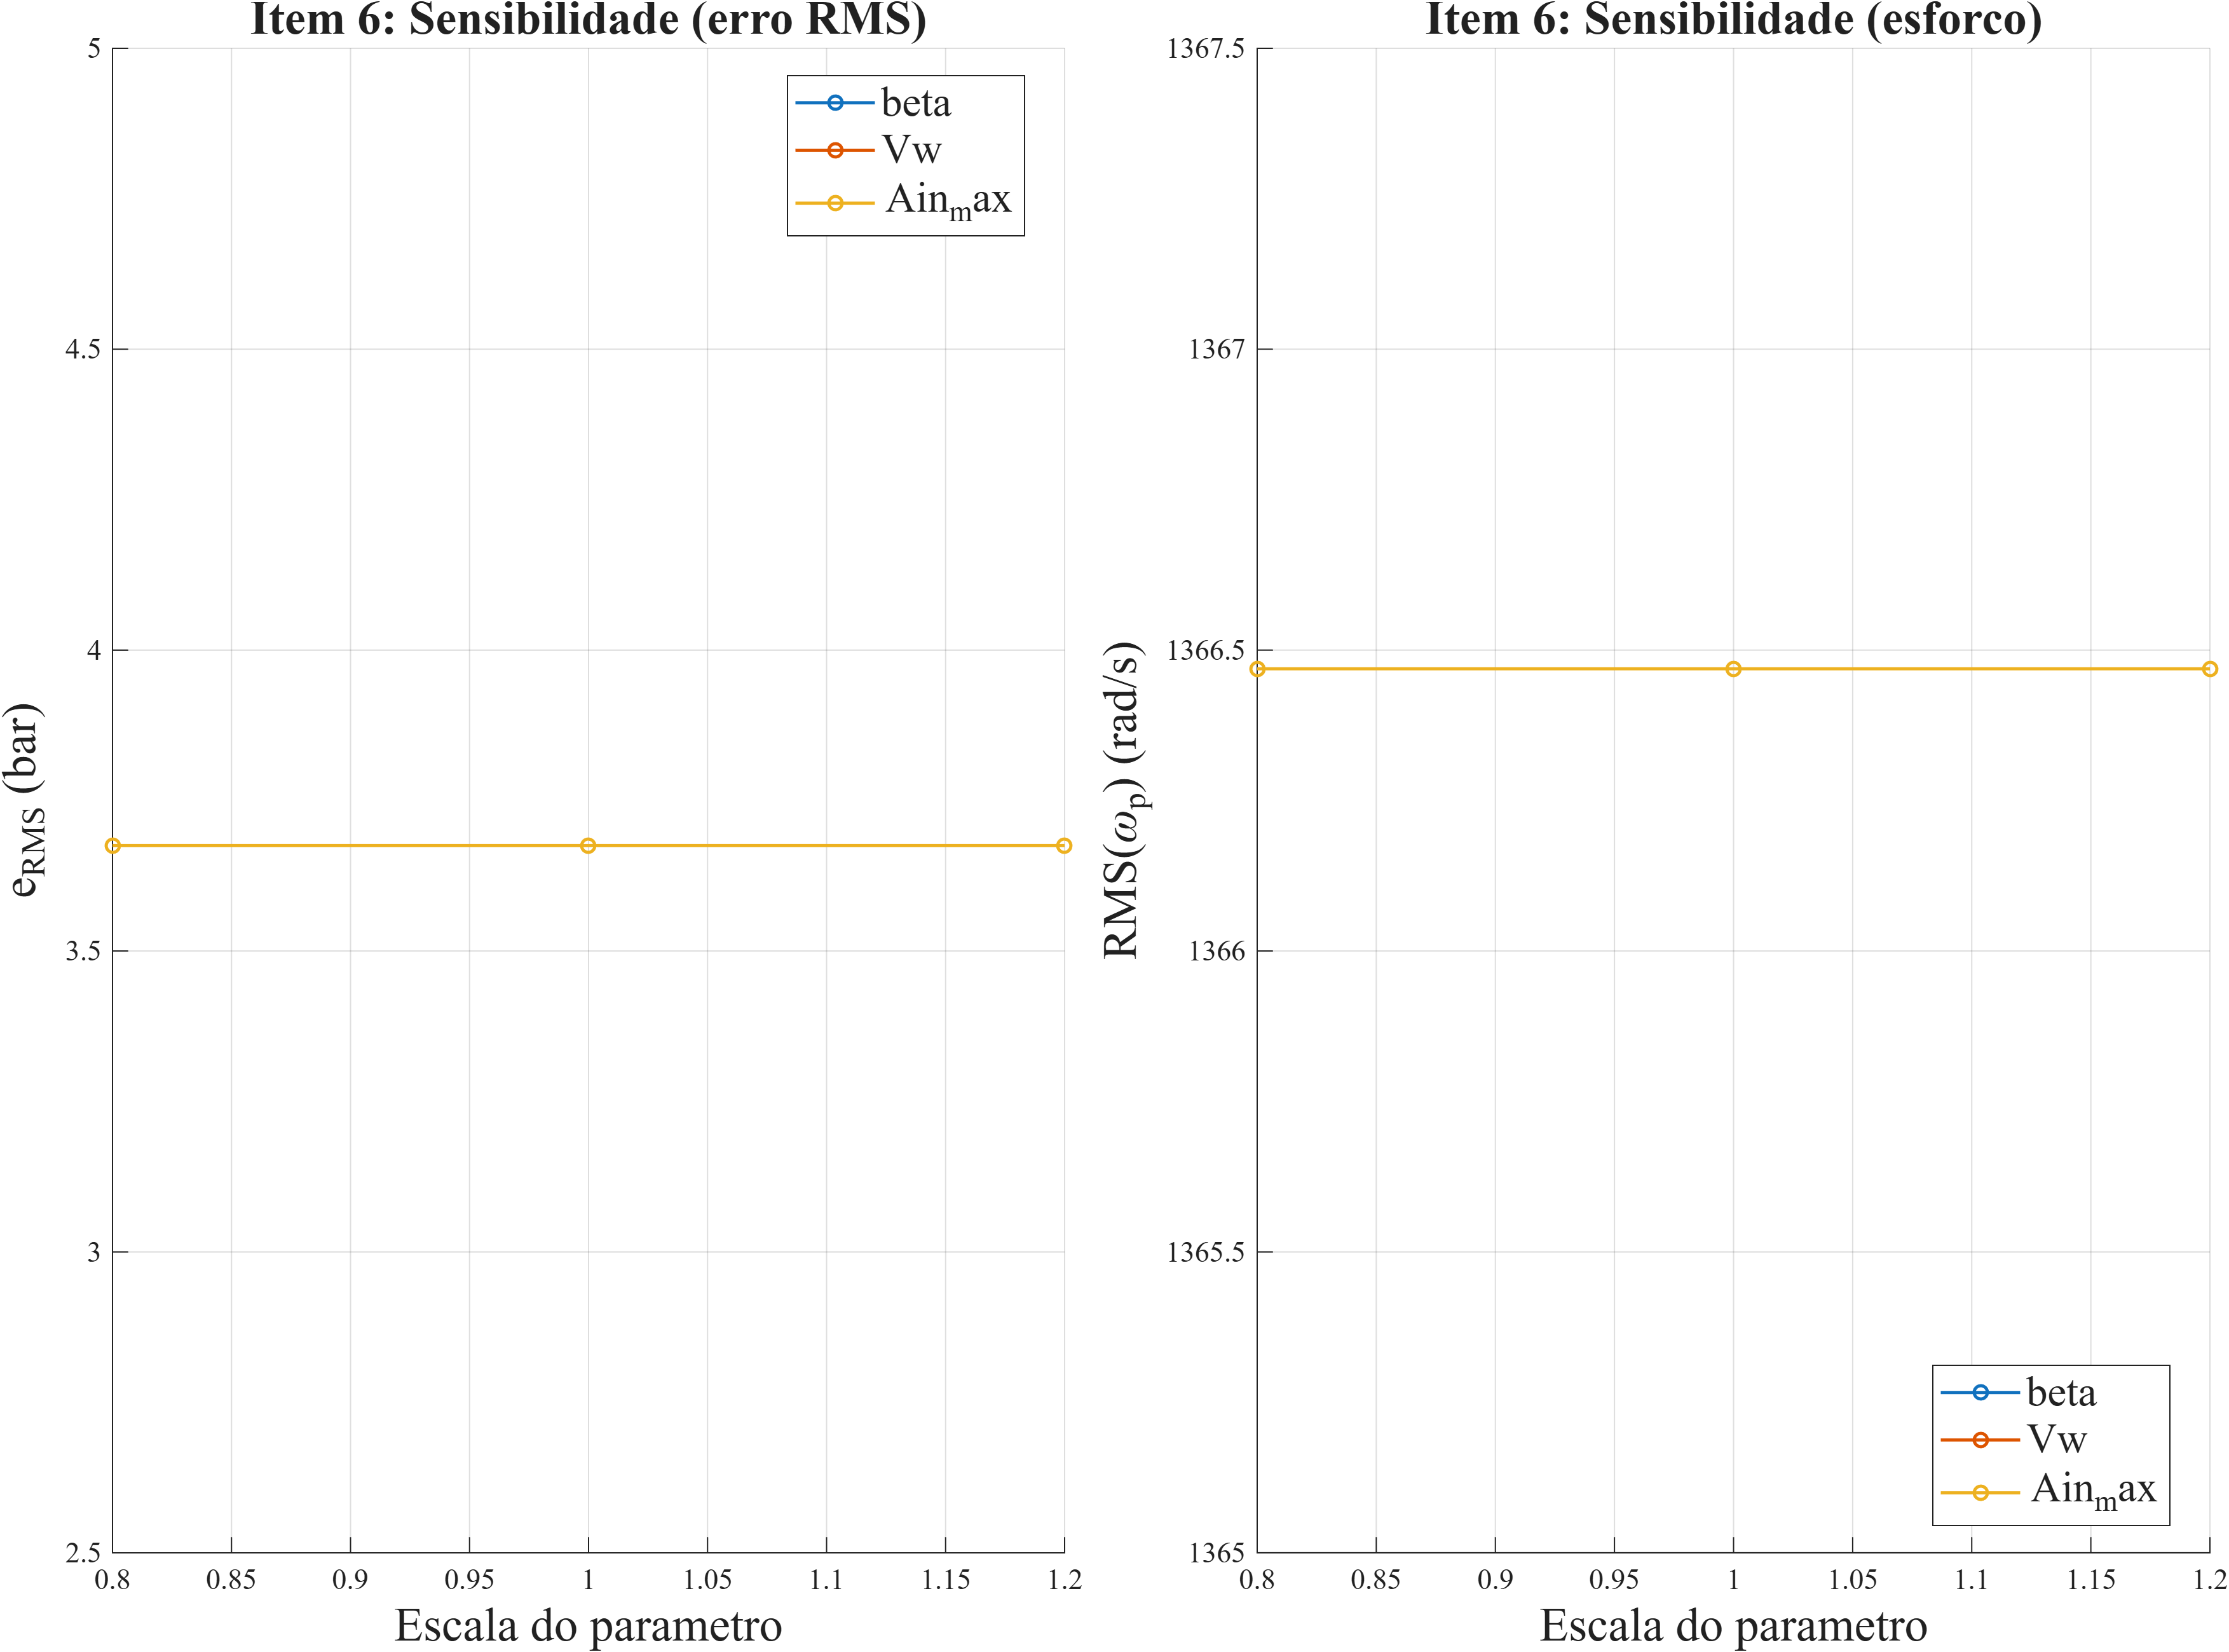
\includegraphics[width=0.92\textwidth]{figuras/artigo_item06_sensibilidade_parametrica.png}
    \Caption{\label{fig:artigo_item06_sensibilidade_parametrica} Sensibilidade paramétrica: impacto em métricas de erro e esforço.}
\end{figure}

Na faixa de variação adotada, a Figura~\ref{fig:artigo_item06_sensibilidade_parametrica} indica degradação moderada de desempenho, sem perda abrupta de seguimento. Esse resultado é compatível com o objetivo desta etapa: discutir robustez prática por simulação, sem afirmar garantias formais para incertezas amplas fora da vizinhança avaliada.

\begin{figure}[htbp]
    \centering
    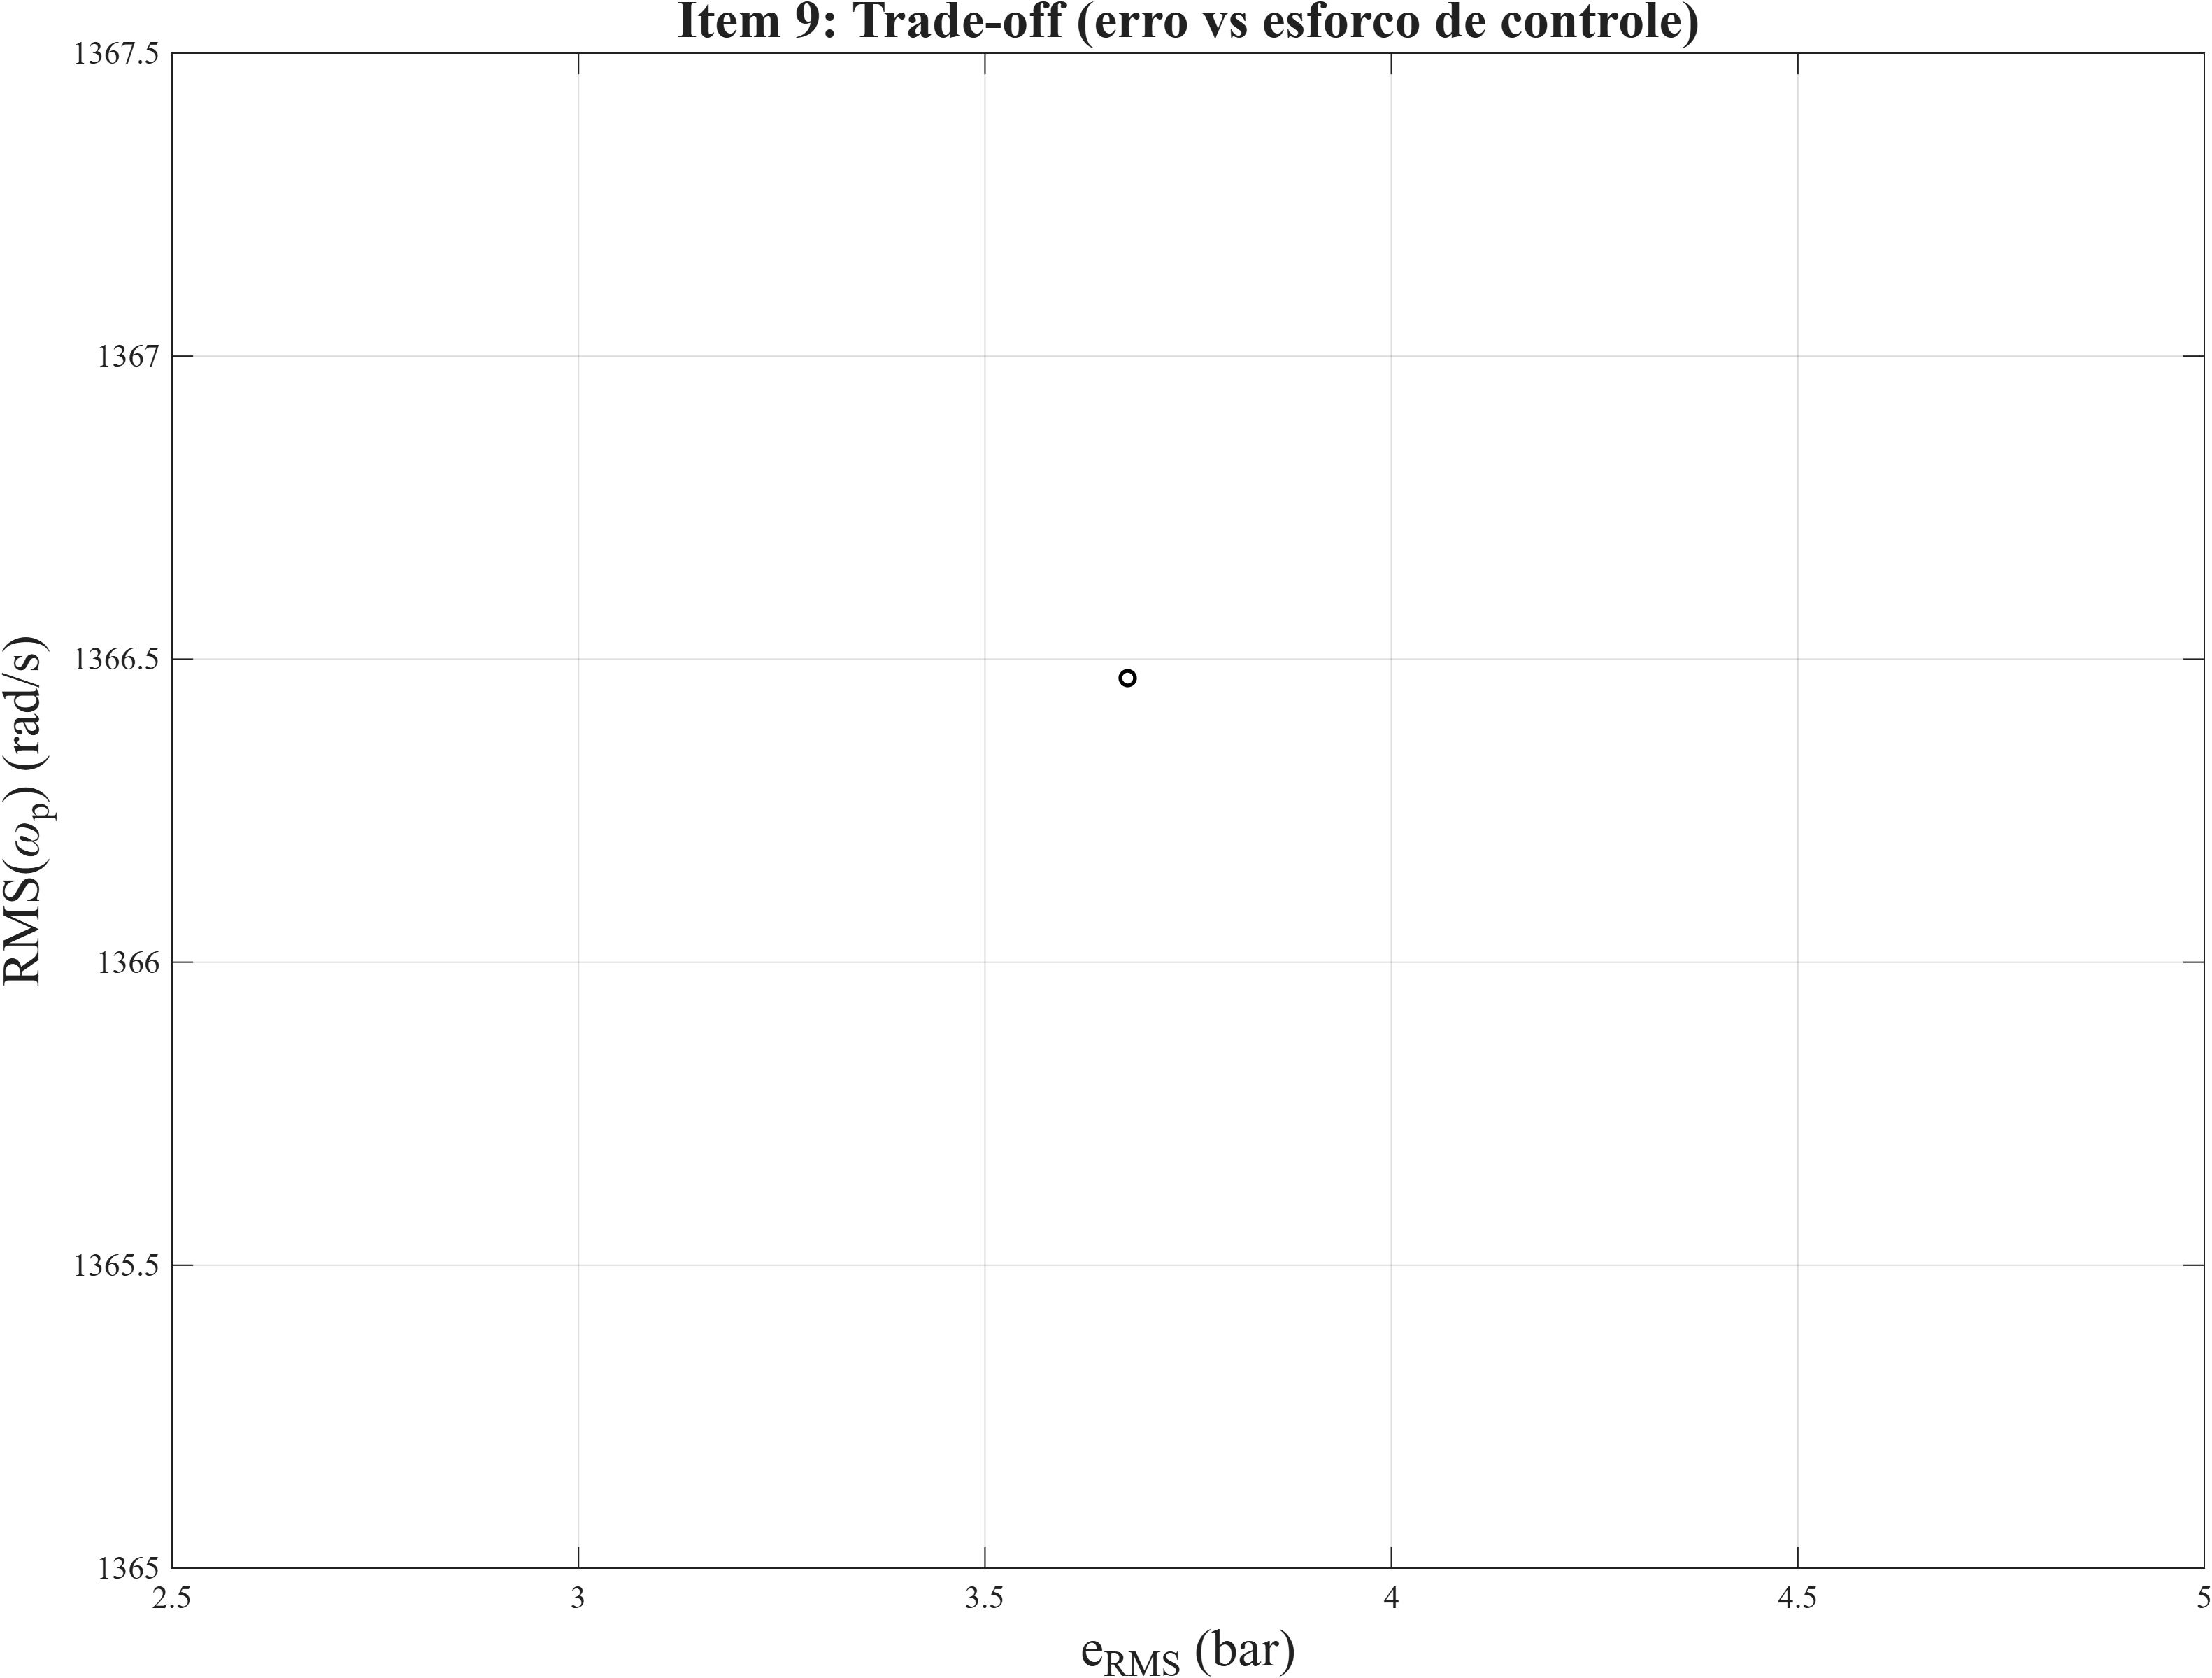
\includegraphics[width=0.92\textwidth]{figuras/artigo_item09_tradeoff_erro_esforco.png}
    \Caption{\label{fig:artigo_item09_tradeoff_erro_esforco} Compromisso erro-esforço para diferentes ponderações de controle.}
\end{figure}

A Figura~\ref{fig:artigo_item09_tradeoff_erro_esforco} explicita que reduzir erro pode elevar esforço de atuação, saturação e atividade de comutação. A inclusão desse gráfico evita conclusões dependentes de uma única escolha de pesos do LQI e torna mais transparente o critério de ajuste adotado no estudo.

\begin{figure}[htbp]
    \centering
    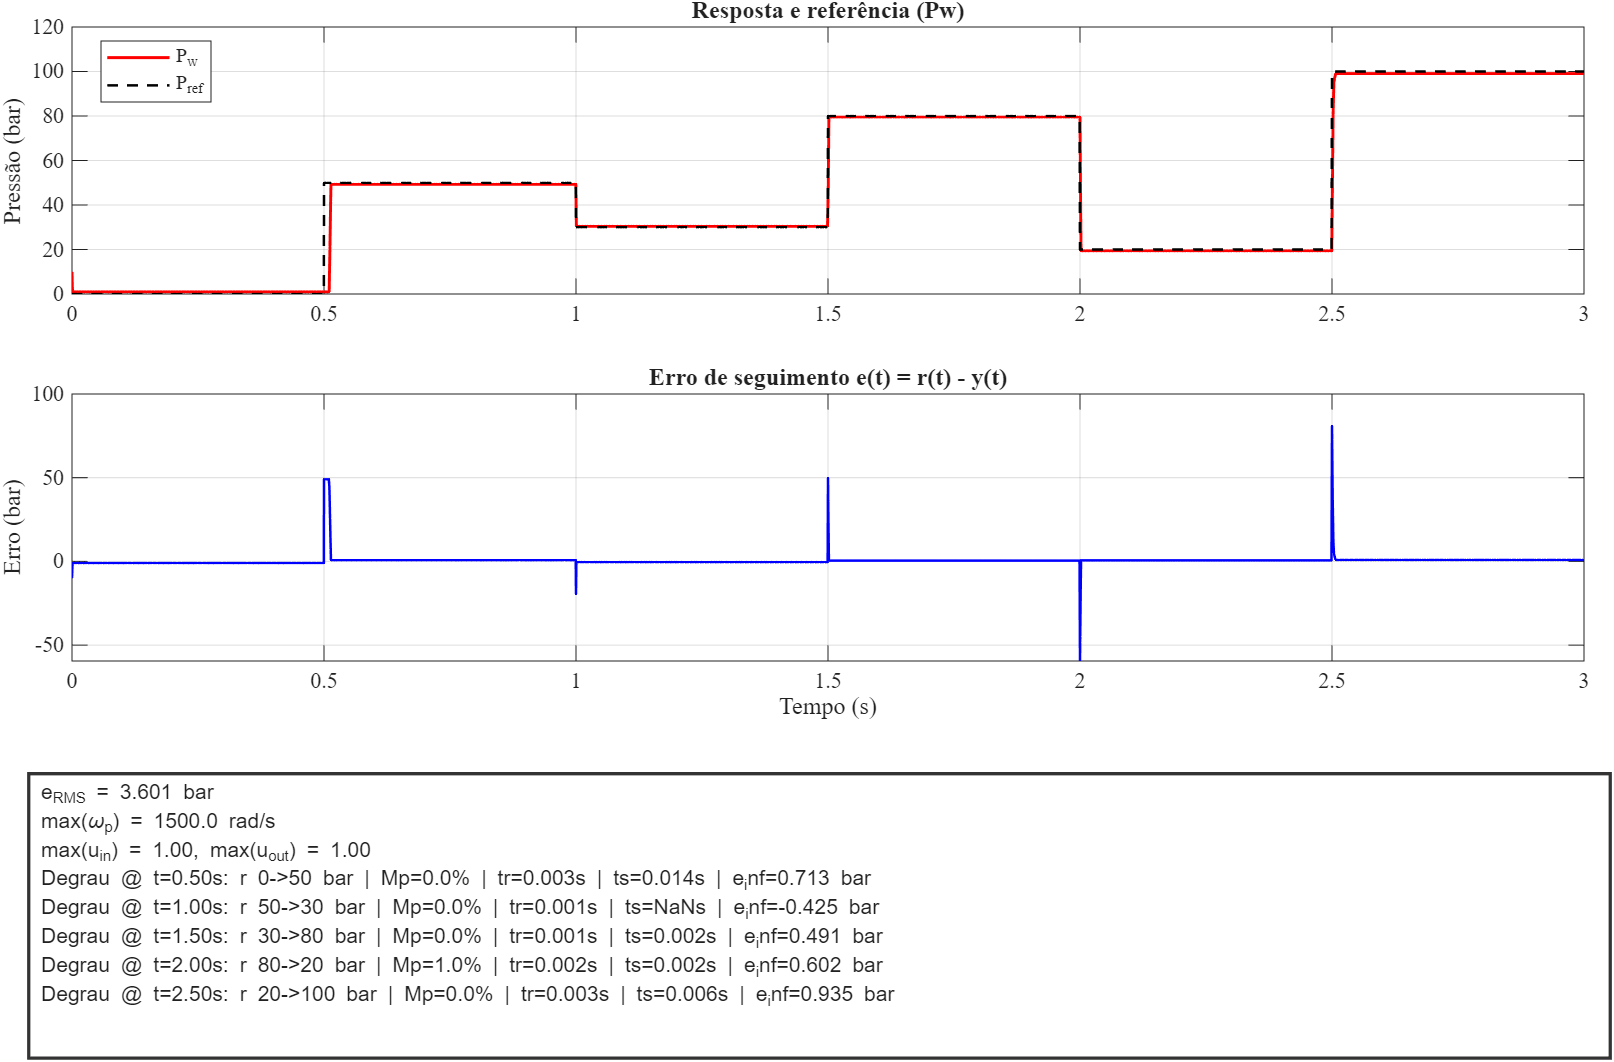
\includegraphics[width=0.92\textwidth]{figuras/metricas_desempenho.png}
    \Caption{\label{fig:metricas_desempenho} Resumo das métricas de desempenho calculadas a partir dos sinais registrados no Simulink para o perfil de referência em patamares.}
\end{figure}

Mesmo quando os valores numéricos dependem dos parâmetros do ensaio, a leitura conjunta das curvas (Figura~\ref{fig:simulacao_comandos_e_pressao}) e do resumo por métricas (Figura~\ref{fig:metricas_desempenho}) fornece um critério objetivo para discutir o compromisso entre \emph{qualidade de seguimento} e \emph{esforço de atuação}. Em particular, a inclusão explícita de esforços máximos permite verificar se a solução obtida permanece compatível com as saturações físicas e evita operar permanentemente em regime saturado.

\section{Sensibilidade a ruído de medição e transições de referência}
\label{sec:resultados-ruido-transicoes}

Para aproximar o cenário de instrumentação real, considera-se a medição de pressão com ruído aditivo na entrada do observador, conforme discutido no Capítulo de Controle. A Figura~\ref{fig:artigo_simulacao_ruido_medicao} apresenta o efeito no domínio do tempo, enquanto a Figura~\ref{fig:artigo_item10_robustez_ruido} sintetiza a degradação de métricas em função do nível de ruído.

\begin{figure}[htbp]
    \centering
    \includegraphics[width=0.92\textwidth]{figuras/artigo_simulacao_ruido_medicao.png}
    \Caption{\label{fig:artigo_simulacao_ruido_medicao} Simulação em malha fechada com ruído de medição em $P_w$.}
\end{figure}

\begin{figure}[htbp]
    \centering
    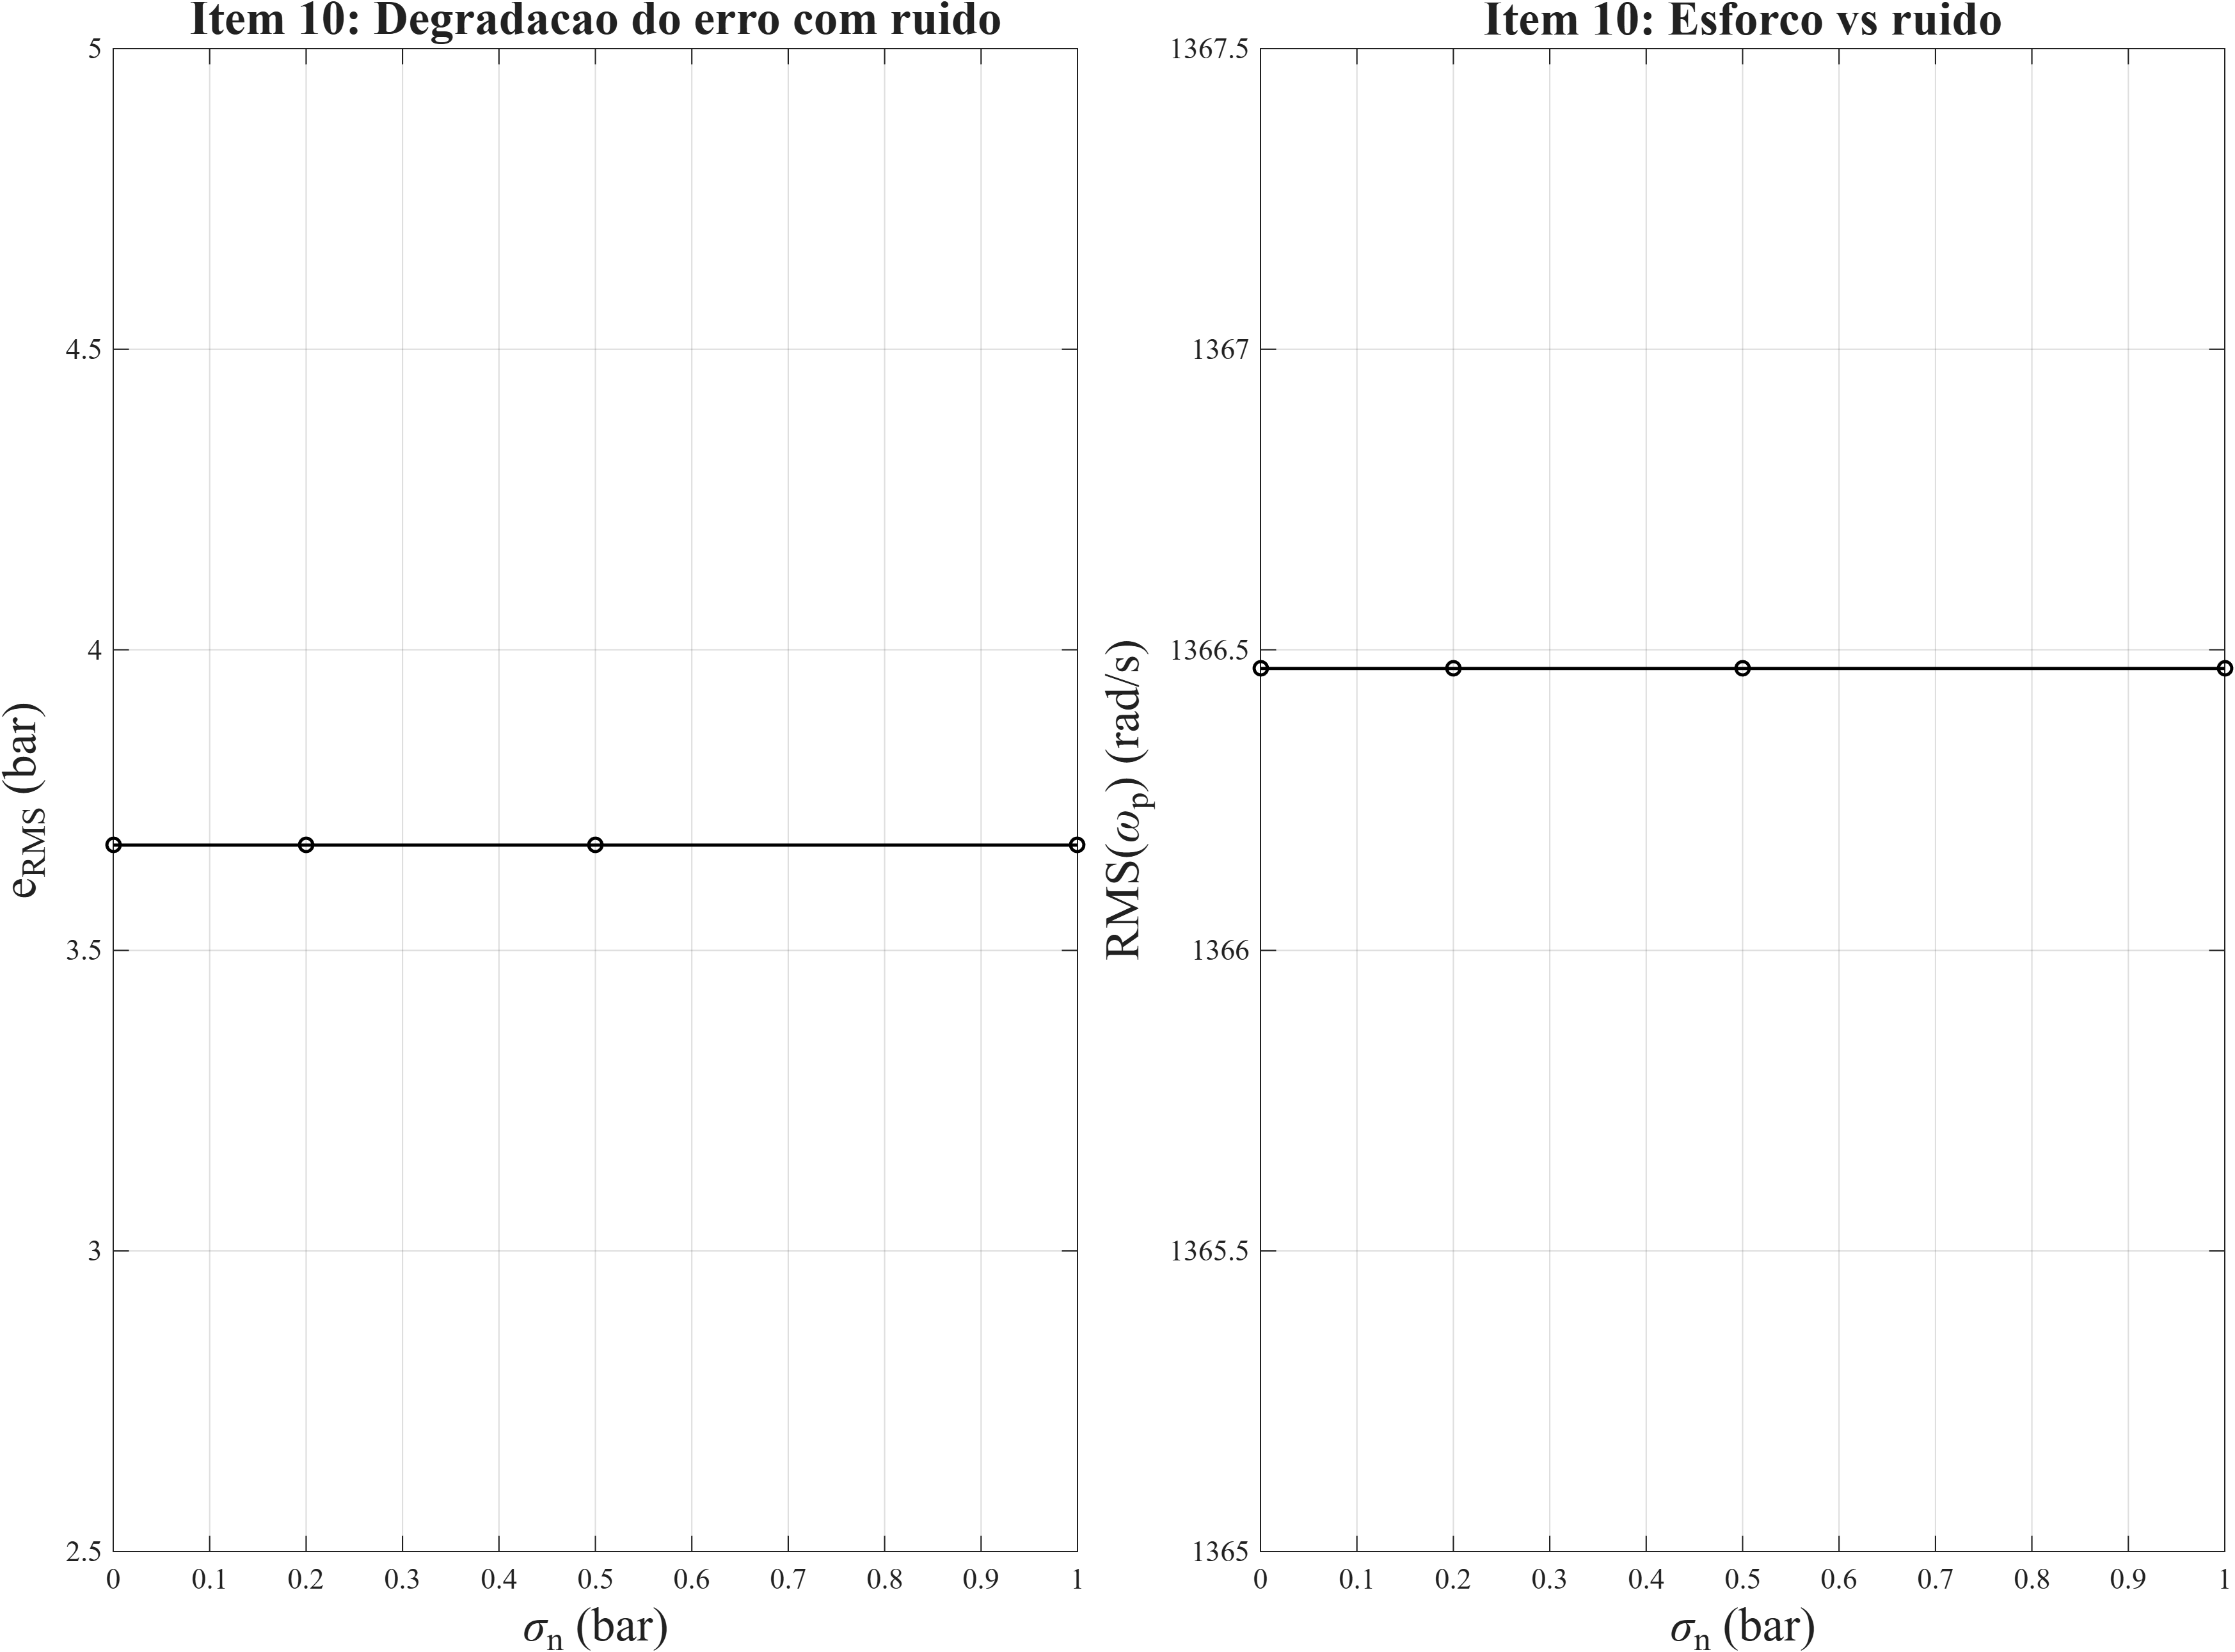
\includegraphics[width=0.92\textwidth]{figuras/artigo_item10_robustez_ruido.png}
    \Caption{\label{fig:artigo_item10_robustez_ruido} Métricas globais de erro e esforço em função do nível de ruído de medição.}
\end{figure}

Na faixa analisada, observa-se aumento gradual de erro RMS e esforço RMS com o crescimento do ruído, sem ruptura abrupta de desempenho. Em termos de engenharia, esse comportamento sugere que o arranjo controlador-observador tolera níveis plausíveis de ruído, ao custo de maior atividade de controle.

Complementarmente, a Figura~\ref{fig:artigo_item11_transicoes_referencia} destaca as regiões de transição de referência e ajuda a separar limitações de rastreamento associadas a degraus agressivos de efeitos de regime em patamar.

\begin{figure}[htbp]
    \centering
    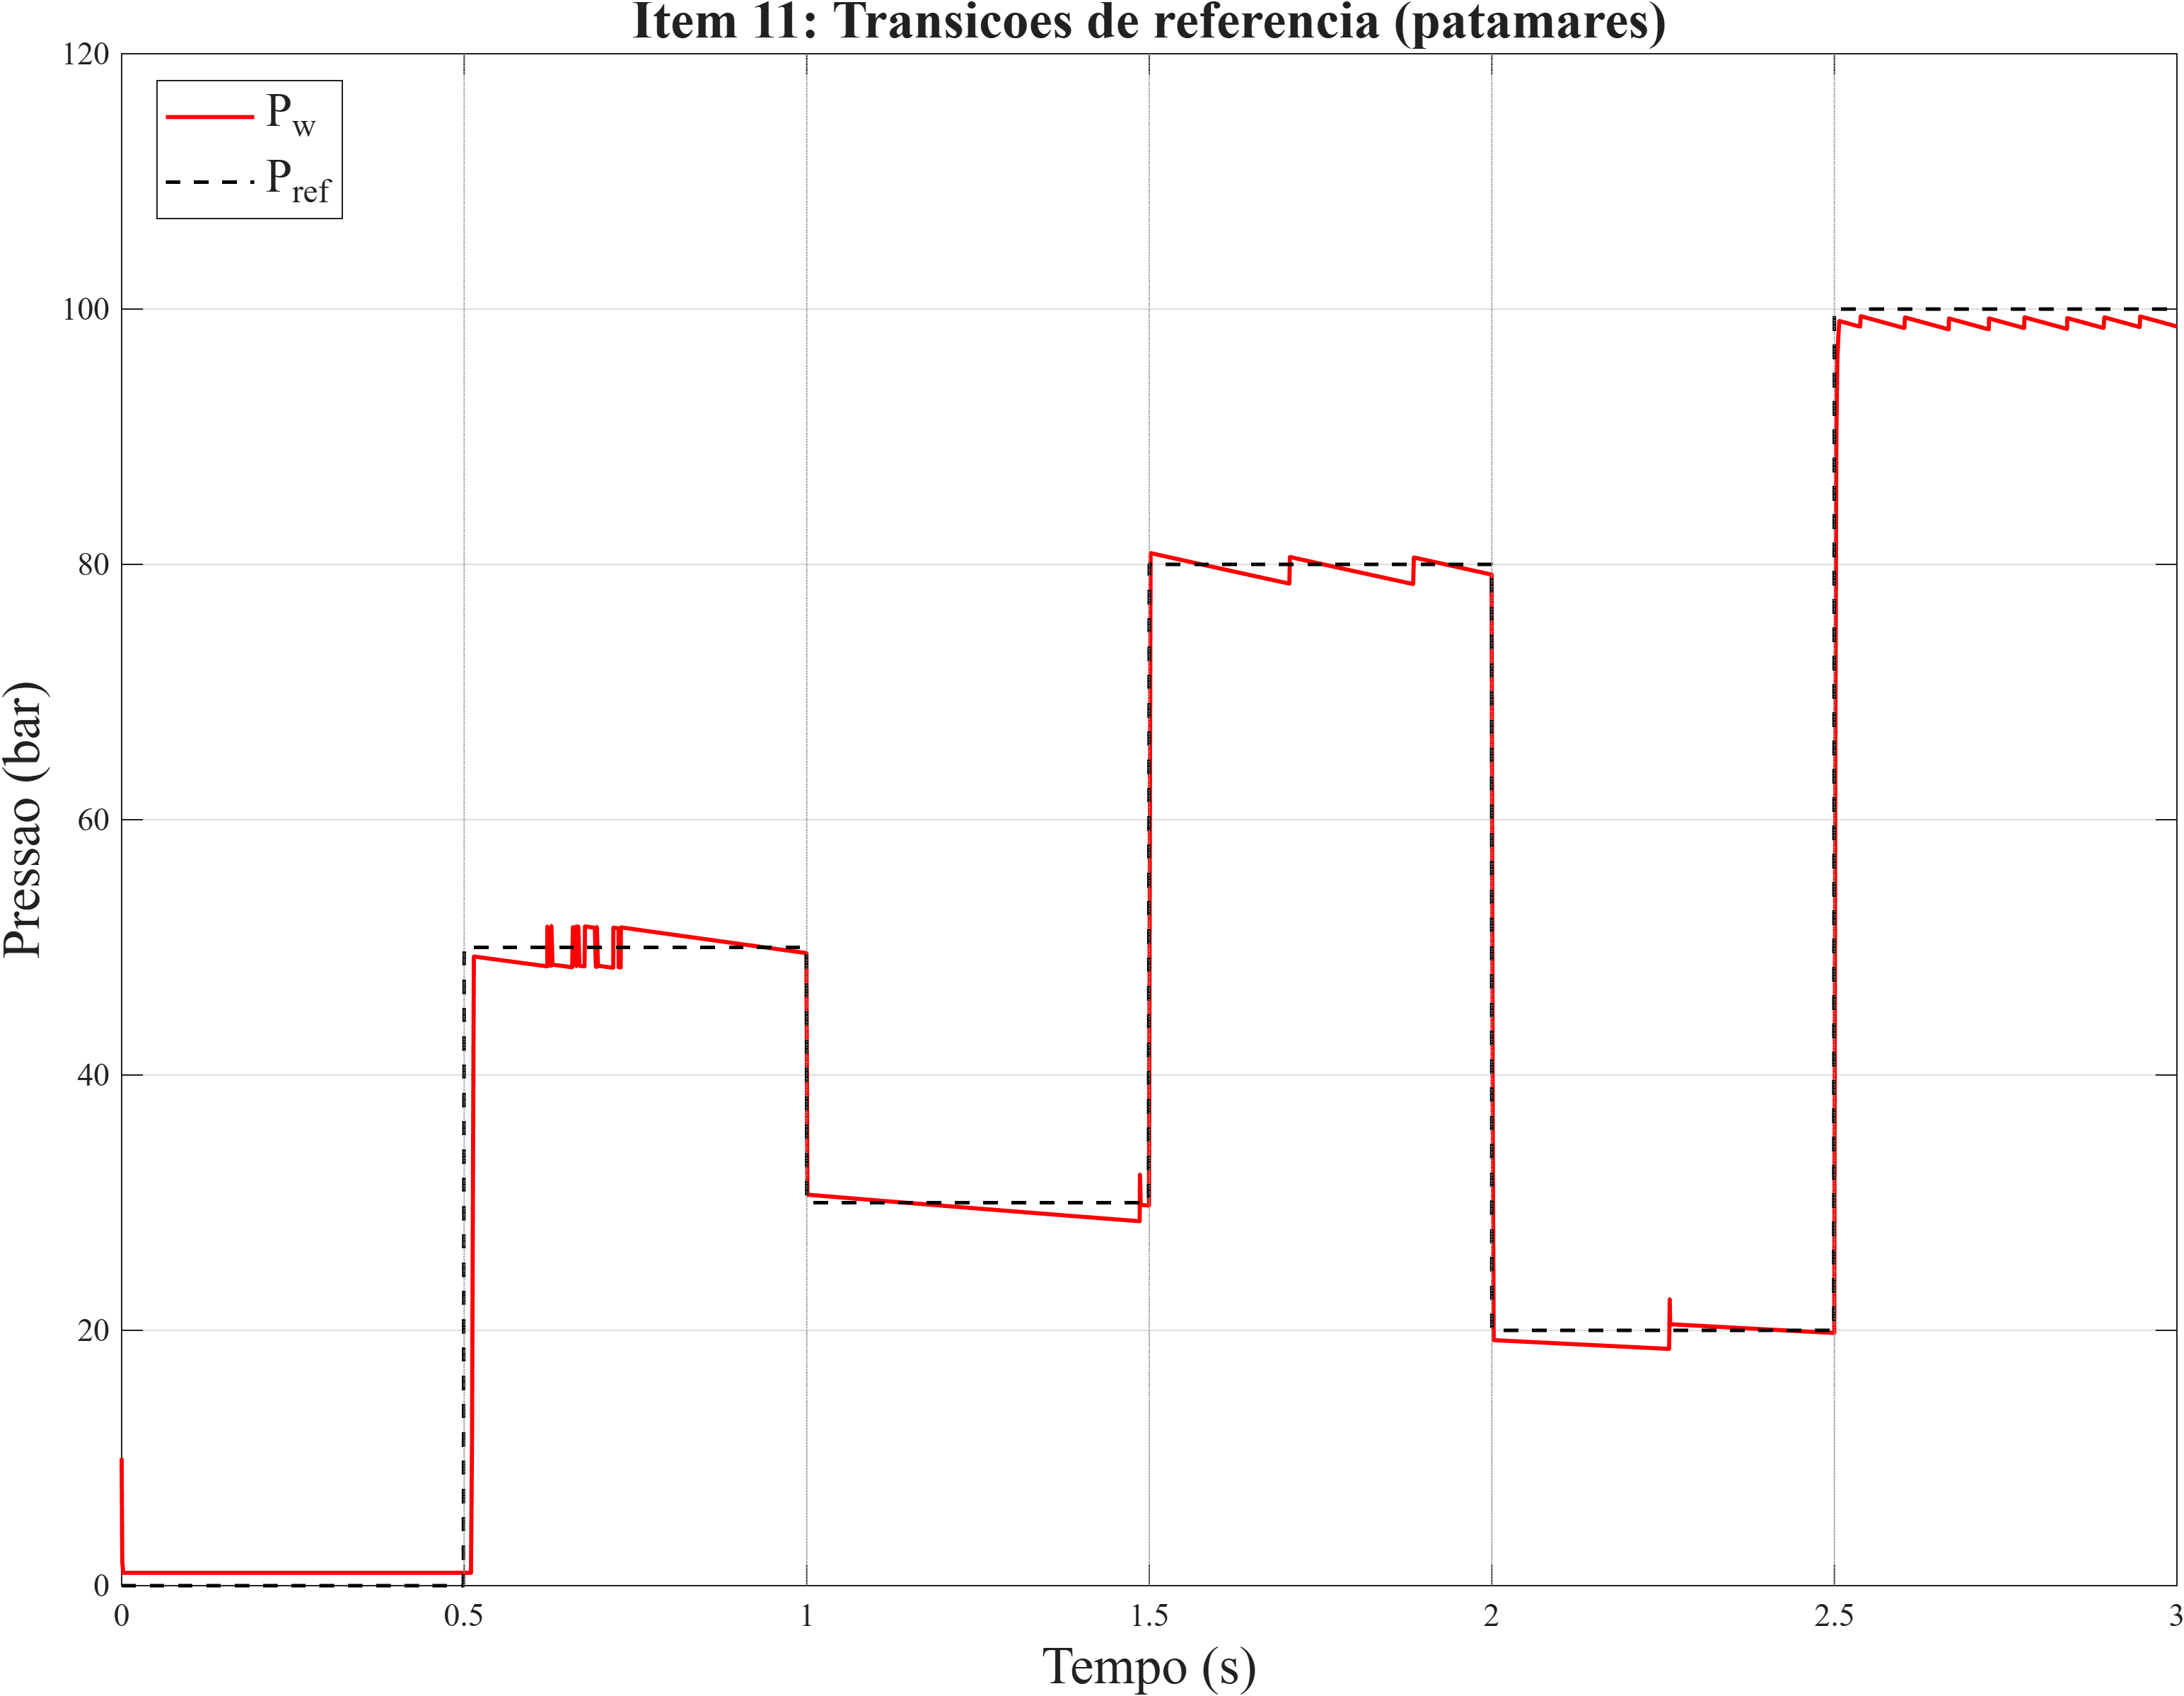
\includegraphics[width=0.92\textwidth]{figuras/artigo_item11_transicoes_referencia.png}
    \Caption{\label{fig:artigo_item11_transicoes_referencia} Destaque das transições de referência e resposta do sistema.}
\end{figure}

\section{Checagens adicionais de plausibilidade}
\label{sec:resultados-plausibilidade}

Como fechamento do conjunto de evidências, a Figura~\ref{fig:artigo_item12_plausibilidade_resumo} reúne indicadores de plausibilidade física e consistência dos resultados simulados, reforçando a interpretação de que o comportamento observado é coerente com o modelo hidráulico adotado e com as restrições explícitas de atuação.

\begin{figure}[htbp]
    \centering
    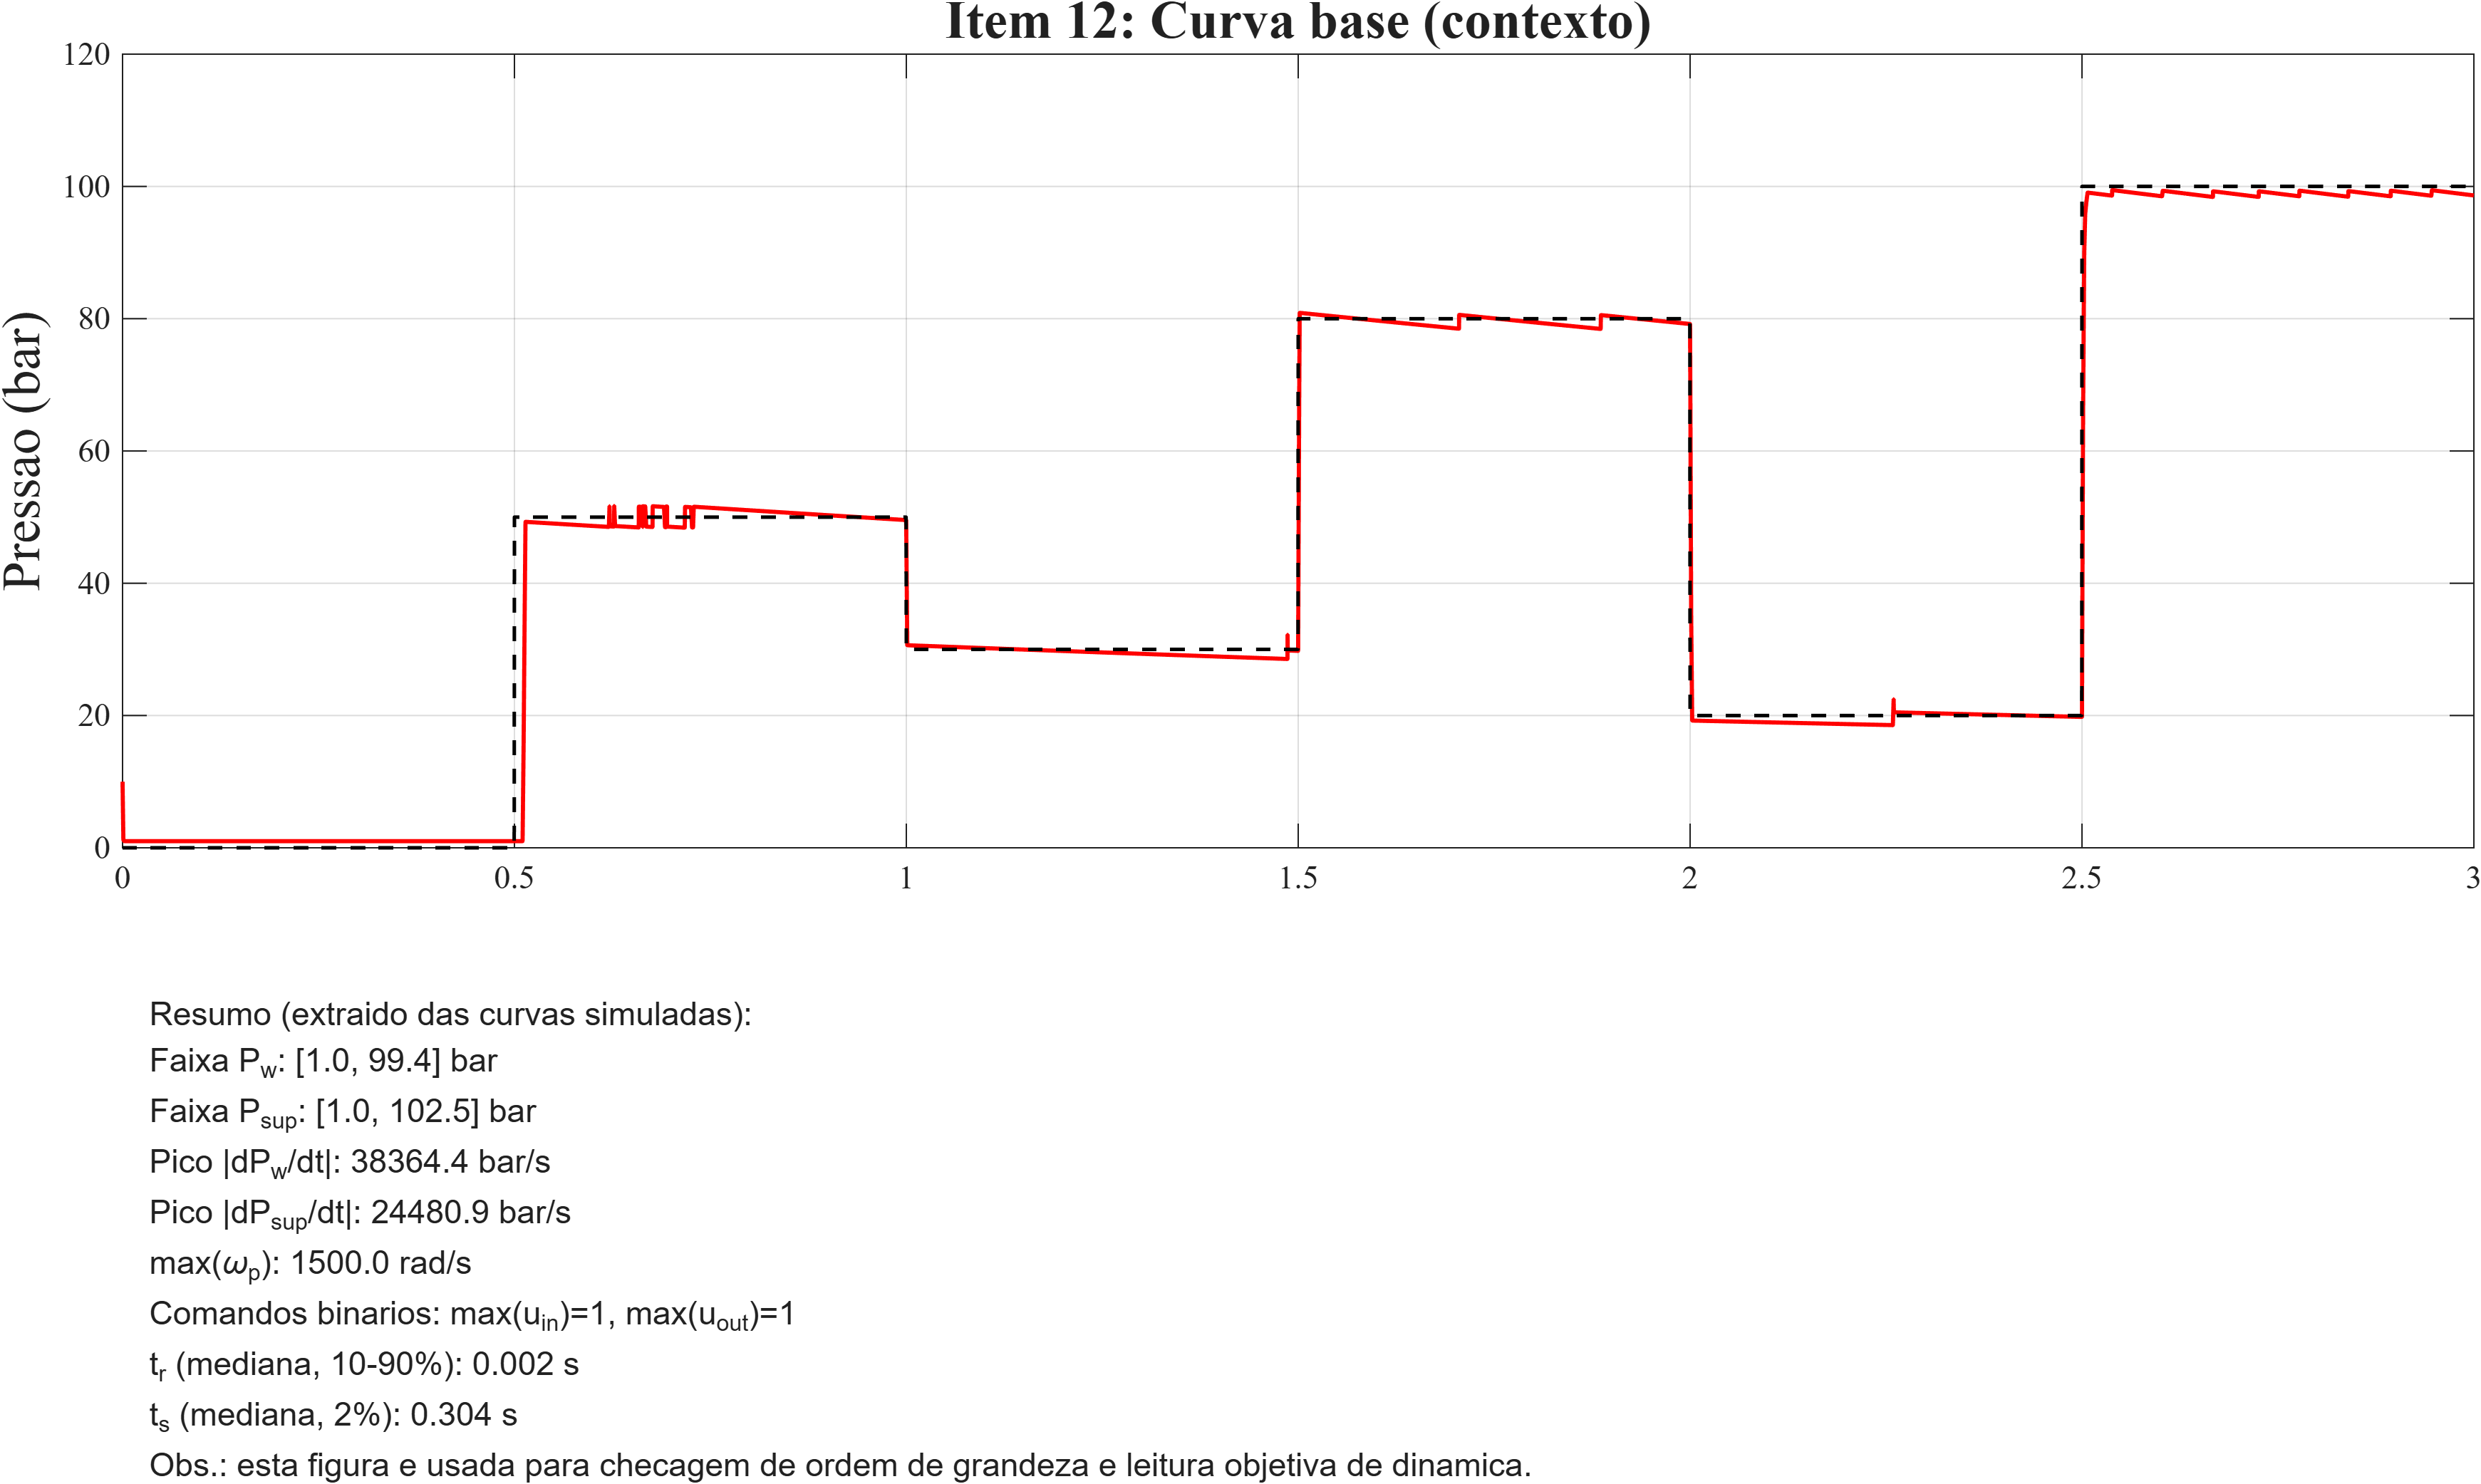
\includegraphics[width=0.92\textwidth]{figuras/artigo_item12_plausibilidade_resumo.png}
    \Caption{\label{fig:artigo_item12_plausibilidade_resumo} Resumo de plausibilidade física e consistência dos ensaios.}
\end{figure}

\section{Desenvolvimento da plataforma experimental}
\label{sec:resultados-plataforma}
Além da validação em simulação, foi desenvolvido um protótipo de placa eletrônica com foco em viabilizar a futura migração da estratégia de controle para execução embarcada e testes em bancada. Trata-se de um resultado de engenharia de suporte ao objetivo principal do trabalho: reduzir a distância entre o controlador validado em Simulink e a implementação em microcontrolador com acionamento de atuadores do modulador.

Embora a validação apresentada neste capítulo seja estritamente em ambiente simulado, a inclusão da plataforma é justificada pelo encadeamento de implementação adotado no Capítulo~\ref{cap:controle}: o controlador discreto opera a partir de uma variável medida de pressão e produz comandos que, em uma arquitetura embarcada, se materializam como sinais de acionamento de bomba e PWM para válvulas. Assim, a plataforma não é apresentada como \emph{evidência} de desempenho do controle (o que exigiria medições em bancada), mas como um elemento de viabilização e rastreabilidade do caminho de transição \textit{model-in-the-loop} $\rightarrow$ \textit{hardware-in-the-loop/bancada}, explicitando a compatibilidade entre a interface de sinais assumida na simulação ($\omega_p$, $u_{in}$, $u_{out}$ e pressão medida) e a instrumentação/acionamento previstos.

\subsection{Impress\~ao e montagem da placa}
\label{sec:resultados-placa}
Como evidência do protótipo, a Figura~\ref{fig:imagem_placa_montada} apresenta uma das placas montadas. Foram impressas 5 placas e todas foram populadas ao menos com os componentes básicos (capacitores e resistores). Dentre elas, 2 possuem montagem completa e 3, até a entrega desta escrita, estão sem o \textit{driver} SB0410 (responsável pelo acionamento de 4 válvulas solenoides).

\begin{figure}[htbp]
    \centering
    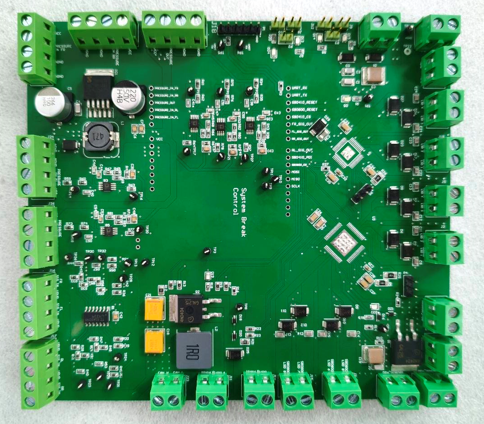
\includegraphics[width=0.82\textwidth]{figuras/imagem_placa_montada.png}
    \Caption{\label{fig:imagem_placa_montada} Protótipo da placa de controle desenvolvida para integração futura com o conjunto de frenagem.}
\end{figure}

\subsection{Arquitetura de integraç\~ao}
\label{sec:resultados-arquitetura}
A arquitetura funcional de integração entre o ambiente de simulação, o controlador e os elementos de atuação/sensoriamento é ilustrada na Figura~\ref{fig:arquitetura-funcional-do-sistema-de-controle-de-freio}. O diagrama resume a visão de sistema adotada: (i) geração de referência e monitoramento, (ii) execução do controle discreto e (iii) interface com sensores e atuadores.

\begin{figure}[htbp]
    \centering
    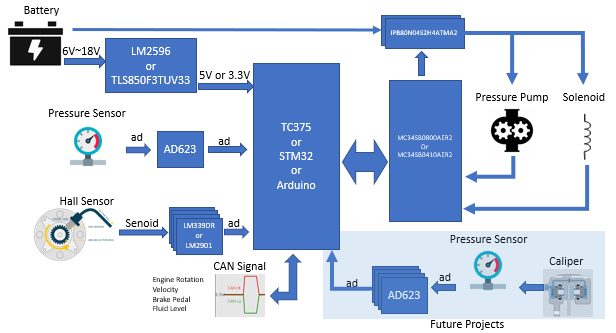
\includegraphics[width=0.92\textwidth]{figuras/arquitetura-funcional-do-sistema-de-controle-de-freio.png}
    \Caption{\label{fig:arquitetura-funcional-do-sistema-de-controle-de-freio} Arquitetura funcional do sistema de controle proposto, destacando a integração entre simulação, controle discreto e plataforma experimental.}
\end{figure}

\section{Limita\c{c}\~oes e trabalhos futuros}
\label{sec:resultados-trabalhos-futuros}
Os resultados apresentados demonstram viabilidade em simulação e maturidade do arcabouço de implementação, mas também delimitam claramente o que ainda precisa ser validado em ambiente físico. Como continuidade direta deste trabalho, destacam-se:
\begin{itemize}
    \item implementação embarcada do controle discreto no microcontrolador (incluindo verificação de tempo de execução e temporização do laço de controle em passo fixo);
    \item integração completa do \textit{driver} de válvulas e verificação elétrica/funcional do acionamento dos atuadores;
    \item validação em bancada com o conjunto de freio, com instrumentação mínima (pressão e, quando aplicável, velocidade) para comparação com os sinais esperados em simulação;
    \item ampliar as análises de robustez para incluir ruídos (sensores, quantização), atrasos e cenários operacionais adicionais, bem como consolidar a validação experimental em bancada/HIL.
\end{itemize}

\subsection{Teste de integração com o conjunto de frenagem}
\label{sec:teste-integracao-frenagem}

A verificação da compatibilidade entre a placa de controle e o conjunto de frenagem foi conduzido um teste preliminar de integração. O objetivo foi assegurar que os sinais de comando gerados pelo controlador discreto pudessem acionar corretamente a bomba e as válvulas, e que as leituras de pressão fossem capturadas de forma consistente.

Para isso, a placa foi conectada ao conjunto de frenagem em um ambiente controlado, e foram aplicados comandos de referência simulados. As respostas de pressão foram monitoradas e comparadas com os valores esperados, permitindo identificar quaisquer discrepâncias ou falhas de comunicação.

A primeira verificação que foi observada é que o bloco hidráulico que foi modelado no Simulink apresentou comportamento diferente do modelo teórico, e isso se deve ao fato de que o modelo teórico possui uma bomba centrífuga. O modelo teórico possui uma pressão de sistema de pelo menos 1e5 Pa, enquanto o modelo real não possui essa pressão, e isso se deve ao fato de que a bomba centrífuga não consegue gerar pressão suficiente para o sistema, ao ponto que ela apenas recircula o fluido.

Neste contexto, foi preciso alterar a bomba do sistema real para uma bomba de deslocamento linear. Esse modelo de bomba desloca um êmbolo que garante assim a pressão necessária para o funcionamento adequado do conjunto de frenagem. Neste modelo, a distância que o êmbolo se desloca é proporcional à velocidade angular do motor que aciona a bomba, e isso garante que a pressão de sistema seja mantida em um nível adequado para o funcionamento do conjunto de frenagem.

Outra observação importante é que o uso do Simulink para gerar os sinais de referência e de comando para a placa, não é o ideal, pois o Simulink funciona em tempo contínuo, e a placa funciona em tempo discreto. Isso gera um problema de sincronização entre os sinais e como a placa envia uma quantidade de dados muito maior que a comunicação USB consegue suportar, gera um \textit{overload} de sinais, fazendo com que os sinais de comando e referência não sejam aplicados corretamente, causando uma instabilidade no sistema, fazendo que o sistema não consiga atingir a pressão desejada, danificando assim o conjunto de instrumentação e as válvulas do conjunto de frenagem, uma vez que o sistema não consegue fazer o desligamento das válvulas de forma adequada, e isso gera o superaquecimento, que danifica as válvulas.

Também, o fato de o driver de válvula SB0410 e SB0800 possuir configuração SPI, mesmo sendo possível implementar a comunicação SPI, no caso do SB0800, para o seu funcionamento, é preciso enviar um sinal contínuo de \textit{watchdog}, e a complexidade de implementar isso no Simulink, mas o tempo de processamento, como foi mencionado anteriormente, gerava atraso na comunicação, e isso fazia com que o driver de válvula não funcionasse corretamente.

A solução mais segura para esse problema foi manter todo o controle do sistema em tempo discreto, e isso foi feito criando os sinais de referência e de comando diretamente na placa, neste novo arranjo, a placa passa a gerar os sinais de referência e de comando, e o Simulink apenas monitora os sinais de pressão, garantindo assim que o sistema funcione de forma adequada, sem sobrecarga de sinais e sem danificar o conjunto de frenagem.

Outro obstáculo encontrado foi o fato de que o conjunto de frenagem possui sensores de pressão que não usa comunicação ou leitura conhecida como I2C, SPI ou ADC, pesquisas indicam que o sensor do bloco utiliza um protocolo conhecido como OSPI, \textit{One-Wire SPI}, \begin{comment} TODO: aqui precisa encontrar uma referencia para este protocole que mostre que esse protocolo é propriedade das frabricantes \end{comment} e isso impossibilita a leitura dos sinais de pressão de suprimento, tornando necessário o desenvolvimento de métodos alternativos para monitorar a pressão no sistema, e neste caso, a modelagem aqui apresentada vai ao encontro e supre a falta deste sensor, uma vez que o modelo de pressão de suprimento pode ser estimado utilizando o deslocamento do êmbolo, garantindo assim que o sistema funcione de forma adequada, mesmo sem a leitura direta do sensor de pressão de suprimento.

Como foi descrito, a alteração do modelo de bomba para uma bomba de deslocamento linear, foi necessária para que o sistema funcione de forma adequada, e que tenha, pelo menos, o mesmo comportamento do modelo teórico, garantindo assim que o sistema funcione de forma adequada, e que seja possivel continuar com a validação do sistema de controle, e que seja possível realizar os testes de bancada. 

Se fez necessario a troca do sistema, nao apenas pelo motivo de que a bomba era centrifuga, mas também pelo fato de que o sistema de frenagem modernos, utilizados em veiculos com tecnologia ADAS, utilizam bombas de deslocamento linear, por ser mais robustas, e por ser mais confiáveis, garantindo assim que o sistema funcione de forma adequada, e que seja possivel continuar com a validação do sistema de controle, e que seja possível realizar os testes de bancada.

para o desenvolvimento dos teste, para o novo sistema, antes de fazer o controle da pressao, foi feito um controle para de malha por segurança do motor. Sem ela, o motor não sabe onde está e pode bater no fim de curso mecânico. Isso não é o objeto de estudo — é infraestrutura. É como o servo de um braço robótico: ele precisa de PID de posição para funcionar, mas o estudo é sobre o que o braço faz, não sobre o servo.

\begin{comment}
#############################################################################################
##############################################################################################
############################################################################################
#############################################################################################
\end{comment}


\section{Teste de Integração com o Conjunto de Frenagem 2.0}

O teste de integração teve como objetivo avaliar o comportamento dinâmico do sistema de frenagem equipado com o atuador linear LAC e validá-lo em condições de operação malha aberta. Substituiu-se o modelo baseado em bomba centrífuga, proposto na modelagem teórica, por uma planta física baseada no acionamento linear do pistão hidráulico.

O ensaio foi projetado para simular um ciclo completo de pressurização em malha aberta, seguido por uma retenção temporária (hold) e subsequente alívio. O teste foi implementado em firmware no microcontrolador AURIX TC375 e os dados coletados foram exportados para processamento e visualização no MATLAB. Abaixo, são descritos os métodos e resultados associados ao experimento.

\subsection{Método Experimental}

O teste consiste em um ciclo de 4,5 segundos composto por três etapas principais:
\begin{itemize}
    \item \textbf{Pressurização:} A válvula principal é acionada no modo \texttt{Apply} e o motor linear do LAC é ativado com um PWM fixo, movendo o pistão até a pressão alcançar o valor alvo de 100 psi. Ao atingir esse limite, o motor é interrompido.
    \item \textbf{Hold:} Após a estabilização da pressão, o sistema mantém a pressão por um período de 1,5 segundos utilizando o modo \texttt{HoldCandidate}, no qual as válvulas IRL e ORL estão fechadas.
    \item \textbf{Alívio:} No estágio final, o sistema entra em modo de \texttt{ReleaseValidated}, onde a válvula ORL é aberta, permitindo o alívio da pressão até aproximadamente 0 psi.
\end{itemize}

Os tempos de cada fase foram configurados conforme segue: \texttt{T\_Idle} = 1,5 s, \texttt{T\_Hold} = 1,5 s, \texttt{T\_Release} = 1,5 s. O PWM atribuído para o acionamento linear do pistão foi de 15\%. Os dados coletados durante o teste incluíram os sinais de pressão no canal hidráulico (\texttt{pw}), posição do pistão (\texttt{pos}), e estados das válvulas (\texttt{u\_in}, \texttt{u\_out}). Esses dados foram registrados a uma frequência de 1 kHz e um resumo serial foi exportado a cada 5 ms durante o ensaio.

\subsection{Resultados Experimentais}

A Figura~\ref{fig:olstep_pressure} apresenta os dados do ensaio com destaque para a variação da pressão (\texttt{pw}), posição (\texttt{pos}) e comandos das válvulas ao longo do tempo.

\begin{figure}[h!]
    \centering
    \includegraphics[width=1.0\textwidth]{figuras/ensaio_olstep_20260911_145243.png}
    \caption{Comportamento do sistema durante o ensaio de integração: curva de pressão (\texttt{Pw}), posição do pistão (\texttt{pos}), e comando das válvulas (\texttt{u\_in}, \texttt{u\_out}) ao longo do tempo.}
    \label{fig:olstep_pressure}
\end{figure}

Os dados obtidos mostram o seguinte comportamento:

\textbf{Fase de pressurização (0–1500 ms):} A pressão (\texttt{pw}) cresce rapidamente com o LAC em acionamento constante por PWM até atingir o patamar de aproximadamente 100 psi. Observou-se um overshoot de cerca de 15 psi (máximo de 115 psi), estabilizando em 100 psi após \textbf{t\textsubscript{settling} = 200 ms}.

\textbf{Fase de retenção (1500–3000 ms):} A pressão estabilizou em torno de 100 psi durante o período de retenção (\texttt{Hold}). Pequenas oscilações abaixo de \textbf{0,5 psi} foram registradas, indicando estabilidade adequada no sistema valvulado.

\textbf{Fase de alívio (3000–4500 ms):} O alívio de pressão foi conduzido pelo acionamento da válvula ORL (\texttt{u\_out = 1}); a queda foi rápida, com a pressão reduzindo de 100 psi para valores próximos de 0 psi em \textbf{t\textsubscript{release} = 420 ms}.



\subsection{Controle em Malha Fechada com Estimação de Pressão via Observador}

Na modelagem teórica apresentada no Capítulo~4, o regulador LQI opera com
realimentação direta da pressão $P_w$ medida por sensor no canal hidráulico.
Essa arquitetura pressupõe a disponibilidade de um transdutor de pressão
instalado junto ao caliper ou na linha de roda --- componente que, na prática
industrial, não é adotado em veículos de produção.

Em moduladores ABS/ESC comerciais, o sensor de pressão é posicionado
internamente ao bloco hidráulico, tipicamente monitorando a pressão de
suprimento ou a pressão do circuito do cilindro mestre. A pressão efetiva
no caliper não é medida; ela é inferida a partir do modelo do circuito
hidráulico e dos comandos aplicados às válvulas. Perdas por compressibilidade
do fluido, variação de temperatura, desgaste de pastilha e presença de ar no
circuito introduzem desvios entre a pressão estimada e a pressão real na
pinça, que o sistema aceita dentro de uma faixa de tolerância operacional.

A planta experimental construída neste trabalho utiliza um atuador linear
(LAC) acoplado a um cilindro hidráulico, substituindo o conjunto bomba
centrífuga e válvulas de modulação. Nessa configuração, a posição do pistão
$x$ é a variável de atuação primária e está diretamente relacionada ao volume
deslocado no circuito. A pressão $P_w$ no caliper resulta da compressão do
fluido contra a rigidez do conjunto pastilha--disco--caliper.

O ensaio de identificação estática (Staircase, Seção~5.8.1) estabeleceu
experimentalmente a relação $P_w = g(x)$ entre deslocamento do pistão e
pressão resultante. Essa curva, embora não linear, é monótona crescente na
região útil e pode ser invertida numericamente para obter a referência de
posição correspondente a uma pressão desejada: $x_{\text{ref}} = g^{-1}(P_{w,\text{ref}})$.

Com base nessa relação, propõe-se uma arquitetura de controle em que a malha
é fechada em \textbf{posição do LAC}, e a pressão $P_w$ é \textbf{estimada}
por um observador de estados, sem participar diretamente da lei de
realimentação. A estrutura adotada é composta por três blocos:

\begin{enumerate}
    \item \textbf{Conversão de referência:} a referência de pressão
    $P_{w,\text{ref}}$ é convertida em referência de posição
    $x_{\text{ref}} = g^{-1}(P_{w,\text{ref}})$ por meio de interpolação
    na curva estática identificada experimentalmente.

    \item \textbf{Regulador LQR com ação integral:} o controlador minimiza
    o erro de posição $e(k) = x_{\text{ref}} - \hat{x}(k)$ e acumula o erro
    em um integrador $z(k)$ para eliminar o desvio estacionário. A lei de
    controle é
    \begin{equation}
        u(k) = -K_x\,[\hat{x}(k) - x_{\text{ref}}] - K_i\,z(k),
    \end{equation}
    em que $u(k)$ representa o duty-cycle do PWM aplicado ao motor do LAC,
    saturado em $[0,\;100\%]$. Os ganhos $K_x$ e $K_i$ são obtidos pela
    solução da equação de Riccati discreta, com a dinâmica do motor
    identificada a partir dos ensaios PWMSWEEP (Seção~5.8.1).

    \item \textbf{Observador de Luenberger:} estima o estado de posição e,
    por extensão, a pressão no caliper:
    \begin{align}
        \hat{x}(k+1) &= a\,\hat{x}(k) + b\,u(k)
                       + L\,[x_{\text{med}}(k) - \hat{x}(k)], \\
        \hat{P}_w(k)  &= g\bigl(\hat{x}(k)\bigr),
    \end{align}
    em que $x_{\text{med}}$ é a posição lida pelo sensor do LAC e $L$ é o
    ganho do observador, dimensionado para convergência 3--5 vezes mais
    rápida que a dinâmica do controlador. A estimativa $\hat{P}_w$ não
    entra na lei de controle; ela é registrada para comparação com a
    medição direta do sensor de pressão.
\end{enumerate}

Essa arquitetura reproduz, na escala da bancada, a condição real dos
moduladores comerciais: a variável de interesse ($P_w$) não é medida no
ponto de aplicação, e sim estimada a partir do modelo e da posição do
atuador. O sensor de pressão instalado na bancada cumpre exclusivamente o
papel de \textbf{validação} --- permite comparar $\hat{P}_w$ com $P_w$
real e quantificar o erro de estimação introduzido por simplificações do
modelo, histerese mecânica e compressibilidade do fluido.

\subsubsection{Estratégia de validação experimental}

Para avaliar o desempenho dessa arquitetura, dois ensaios comparativos são
conduzidos utilizando o mesmo perfil de referência (degrau de 0 a 100\,psi
com retenção e alívio, conforme Seção~5.8.1):

\begin{itemize}
    \item \textbf{Ensaio~A --- Malha fechada em $P_w$ (referência direta):}
    o controlador recebe $P_w$ medida pelo sensor de pressão como
    realimentação. Serve como caso de referência (melhor desempenho
    alcançável com a instrumentação disponível).

    \item \textbf{Ensaio~B --- Malha fechada em $x$ com observador:}
    o controlador opera sobre a posição estimada $\hat{x}$ e a pressão
    $\hat{P}_w = g(\hat{x})$ é registrada. O sensor de pressão não
    participa da malha; seus dados são usados apenas em pós-processamento
    para calcular o erro de estimação $e_P = P_w - \hat{P}_w$.
\end{itemize}

A comparação entre os dois ensaios permite quantificar a degradação de
desempenho introduzida pela substituição do sensor de pressão pelo
observador, em termos de erro RMS de seguimento, sobressinal, tempo de
acomodação e erro estacionário --- as mesmas métricas utilizadas na
validação em simulação (Seção~5.3).

Essa abordagem tem duas vantagens práticas. Primeiro, demonstra que o
sistema é capaz de operar sem sensor de pressão no caliper, condição
obrigatória em aplicações veiculares. Segundo, fornece dados experimentais
para calibrar e validar o modelo $g(x)$, identificando as faixas de
operação em que a estimação é aceitável e aquelas em que as não
linearidades da planta degradam a precisão além do tolerável.


TESTE




\begin{figure}[h!]
    \centering
    \includegraphics[width=1.0\textwidth]{figuras/ensaio_clstepB_20260912_083523.png}
    \caption{Comportamento do sistema durante o ensaio de integração: curva de pressão (\texttt{Pw}), posição do pistão (\texttt{pos}), e comando das válvulas (\texttt{u\_in}, \texttt{u\_out}) ao longo do tempo.}
    \label{fig:clstep_pressure}
\end{figure}

A Figura~\ref{fig:clstep_pressure} mostra o comportamento do sistema durante o ensaio de integração, incluindo a curva de pressão (\texttt{Pw}), a posição do pistão (\texttt{pos}) e os comandos das válvulas (\texttt{u\_in}, \texttt{u\_out}) ao longo do tempo.

CLSTEP B (LQR em posição) — excelente resultado
Tempo de subida: 98ms (10%→90% de 100 psi)
Sobressinal: 3.8% (103.85 psi)
Erro estacionário: 7.14 psi (Pw≈93 psi vs ref=100)
Estabilização: ~400ms e depois decai lentamente de 103→93 psi
Funciona porque o controlador de posição sabe exatamente onde ir (xRef≈6.85mm), vai rápido (u≈77%), e quando chega perto entra em Hold. A pressão é consequência da posição — e a posição é bem controlada.

O decaimento lento (103→93 psi ao longo de 2s com posição fixa em 6.82mm) é relaxação viscoelástica do fluido/vedações — comportamento físico real, não erro do controlador. O xRef seria ~6.95mm para 100 psi, mas o Hold trava em 6.82mm → a pressão estabiliza um pouco abaixo.



\begin{comment}
#####################################################################################################
#####################################################################################################
#####################################################################################################
#####################################################################################################
#####################################################################################################
#####################################################################################################
\end{comment}











\section{Introdução}
Este trabalho apresenta o desenvolvimento, implementação e validação de um controlador digital em espaço de estados, com realimentação de estados por LQR e observador de Luenberger, aplicado a um módulo hidráulico automotivo MK~C2. A variável de interesse é a pressão na roda (Pw), porém a malha de controle é fechada exclusivamente com a posição do atuador linear (LAC). A pressão é utilizada para identificação, avaliação de desempenho e segurança. A abordagem é, portanto, um controle indireto de pressão via deslocamento.

\section{Planta, Instrumentação e Bancada}
A bancada de frenagem integra:
- Atuador LAC com sensor de posição (encoder) em milímetros.
- Circuito hidráulico com válvulas Apply/Hold/Release e sensor de pressão (psi).
- Eletrônica de comando com amostragem em Ts = 1~ms e registro em duas vias: serial (5~ms) e buffer 1~kHz.

Sinais logados:
- t\_ms (tempo), pos\_mm (posição), pwm\_pct (comando do motor), pw\_psi (pressão), estados de máquina (fase/step).

\section{Procedimentos Experimentais}
Três ensaios foram conduzidos para levantar a dinâmica e calibrar a relação posição–pressão:
\subsection{PWMSWEEP}
Varredura de PWM em degraus constantes, com registro de pos\_mm e pwm\_pct. Objetivo: extrair ganho de velocidade (mm/s por \%PWM) e observar saturações e não linearidades.

\subsection{OLSTEP/PLID}
Pressurização em malha aberta do motor com PWM fixo e transição para Hold no alcance de alvos de pressão. Objetivo: medir pares (pos, Pw) nos patamares de 100, 200 e 300~psi, distinguindo posição de cruzamento (dinâmica) e posição de equilíbrio em Hold (estática).

\subsection{CLMULTI}
Perfil composto 0–100–200–50–0~psi, com controle indireto (posição). Objetivo: avaliar seguimento de referência com segmentos ascendentes e descendentes, métricas por segmento (eRMS, eSS, Mp), overshoot e atuação das válvulas.

\begin{figure}[h]
  \centering
  % Inserir gráfico PWMSWEEP: PWM vs tempo; posição vs tempo; velocidade (derivada suavizada).
  % Comentário: A figura deve mostrar janelas de PWM constante (>5%), com as respectivas curvas de pos(t) e v(t). Destacar a convergência da velocidade a Vss em cada janela, usada para estimar K_vel e tau.
  \caption{PWMSWEEP — janelas de PWM constante e resposta de posição/velocidade.}
  \label{fig:pwmsweep}
\end{figure}

\begin{figure}[h]
  \centering
  % Inserir gráfico PLID: pressão e posição vs tempo para três degraus (100/200/300 psi), com indicação de cruzamento e hold.
  % Comentário: A figura deve evidenciar os três patamares, marcando (pos_cruzamento, Pw_alvo) e (pos_hold, Pw_hold). Usar cores distintas por patamar e tempo relativo para sobrepor as curvas.
  \caption{PLID — três degraus (100/200/300~psi): cruzamento e equilíbrio em Hold.}
  \label{fig:plid}
\end{figure}

\begin{figure}[h]
  \centering
  % Inserir gráfico CLMULTI: Pw_real, Pw_est, pos_mm, Pref e u(%), com métricas por segmento.
  % Comentário: A figura deve apresentar o seguimento por segmento: Idle, 100, 200, 50 e 0 psi; indicar Mp, eRMS e eSS por segmento na legenda/tabela associada.
  \caption{CLMULTI — perfil 0/100/200/50/0~psi: dados serial e buffer 1~kHz.}
  \label{fig:clmulti}
\end{figure}

\section{Modelagem e Identificação}
A dinâmica do atuador e transmissão foi aproximada por
\begin{equation}
  G(s) \;=\; \frac{K}{s(\tau s + 1)}\,,
\end{equation}
onde $K$ é o ganho (mm/s por \%PWM) e $\tau$ a constante de tempo do primeiro polo associado ao motor/estrutura. O termo $1/s$ representa o integrador mecânico da posição.

A identificação utilizou os dados PWMSWEEP e OLSTEP:
- Seleção de janelas de PWM aproximadamente constante (>5~\%) por variância móvel.
- Derivada de posição via filtro de Savitzky–Golay para estimar velocidade $v(t)$.
- Ajuste $v(t) = V_{ss}(1 - e^{-(t-t_0)/\tau})$ nos 600~ms iniciais de cada janela, via mínimos quadrados.
- Cálculo de $K_{\text{vel}} = V_{ss}/u$ (mm/s por \%PWM) e agregação ponderada por $1/\text{RMSE}$.

\begin{figure}[h]
  \centering
  % Inserir gráfico de identificação: v(t) medido vs v̂(t) ajustado em uma janela representativa.
  % Comentário: Mostrar o ajuste exponencial no trecho inicial, com Vss, tau e RMSE anotados; incluir PWM da janela.
  \caption{Ajuste de $v(t)$ em janela de PWM constante para extração de $\tau$ e $K_{\text{vel}}$.}
  \label{fig:id}
\end{figure}

A discretização (ZOH) com $T_s = 1$~ms produziu $(\Phi, \Gamma)$ do modelo em espaço de estados:
\[
  \begin{bmatrix} \dot{x}_1 \\ \dot{x}_2 \end{bmatrix}
  =
  \underbrace{\begin{bmatrix} -\frac{1}{\tau} & 0 \\ 1 & 0 \end{bmatrix}}_{A}
  \begin{bmatrix} x_1 \\ x_2 \end{bmatrix}
  +
  \underbrace{\begin{bmatrix} \frac{K}{\tau} \\ 0 \end{bmatrix}}_{B} u, 
  \quad y = \begin{bmatrix} 0 & 1 \end{bmatrix} \begin{bmatrix} x_1 \\ x_2 \end{bmatrix},
\]
com $x_1$ proporcional à velocidade e $x_2$ à posição. Aplicou-se $[\Phi,\Gamma] = \text{c2d}(A,B,T_s)$.

% Comentário: Incluir tabela com os valores identificados de tau e K_vel (com incerteza), e faixas de operação (PWM baixo/alto). 

\section{Projeto do Controlador (LQR + Integrador)}
\subsection{Estrutura de Controle}
O servossistema em espaço de estados foi implementado com integrador do erro de posição (referência em mm) e realimentação de estados:
\begin{align}
  v[k+1] &= v[k] + \big(x_{\text{ref}}[k] - y[k]\big), \\
  u[k]   &= -K\,\hat{x}[k] + K_i\,v[k],
\end{align}
onde $\hat{x}[k]$ é a estimativa do estado pelo observador. O par $(K, K_i)$ foi projetado via alocação de polos no sistema aumentado (método \emph{acker}), garantindo margem de fase adequada e tempo de acomodação compatível com a dinâmica hidráulica. O pré-filtro foi dispensado, pois a referência é convertida por LUT inversa $g^{-1}$ de psi para mm.

\subsection{Observador de Luenberger}
O observador discreto foi obtido por \emph{place} com polos 2–5 vezes mais rápidos que os polos de malha fechada:
\begin{equation}
  \hat{x}[k+1] \;=\; \Phi\,\hat{x}[k] + \Gamma\,u[k] \;+\; L\big(y[k]-C\,\hat{x}[k]\big).
\end{equation}
A saída medida é a posição ($C = [0\;1]$). A velocidade é estimada pelo observador para evitar derivadas ruidosas.

\subsection{Anti-Windup e Saturações}
Implementou-se anti-\emph{windup} por congelamento do integrador quando $u$ satura nos limites de PWM (e/ou em região de descida com válvula Release). A atuação das válvulas é coordenada pela lógica de trajetória:
- Subida (Pref ascendente): Apply contínuo; o PWM do motor posiciona o LAC.
- Banda de manutenção: tolerância em posição compatível com a oscilação elástica do fluido.
- Descida (Pref descendente): trajetória de $x_{\text{ref}}$ reduzida; motor reduz PWM a zero; a válvula Release auxilia a desacoplar a pressão sem fechar malha com Pw.

\section{Calibração $g(x)$ e LUT inversa $g^{-1}$}
O PLID forneceu pares (pos, Pw) em duas condições:
- Cruzamento (dinâmica): posição no instante em que Pw atinge o alvo.
- Equilíbrio (estática): posição média durante Hold.

Para controle indireto, a LUT $g^{-1}$ privilegia posições de equilíbrio para minimizar os ciclos limites na manutenção. A região alta (6{,}4–7{,}3~mm) é íngreme: pequenas variações de posição causam grandes variações de pressão; a LUT foi suavizada e mantida monotônica. A atualização da LUT foi feita apenas com pontos medidos (PLID e logs CLMULTI), evitando extrapolações.

\begin{figure}[h]
  \centering
  % Inserir gráfico LUT: Pw=f(x) e g^{-1}(Pref) sobre a faixa 6,0–7,4 mm com pontos medidos e ajuste monotônico.
  % Comentário: Mostrar pontos PLID (cruzamento e hold) e a curva escolhida para g e g^{-1}, destacando a faixa íngreme.
  \caption{Curva calibrada $g(x)$ e LUT inversa $g^{-1}$ (pos~→~psi e psi~→~pos).}
  \label{fig:lut}
\end{figure}

\section{Resultados}
As métricas por segmento no CLMULTI foram calculadas a cada perfil:
- eRMS: erro quadrático médio em psi.
- eSS: erro em regime em psi.
- $M_p$: máximo sobressinal em \%.

Observou-se:
- Subida a 100~psi: seguimento com banda reduzida e mínima oscilação quando a banda de posição foi ajustada para refletir a compressibilidade (redução do ciclo limite).
- Transição a 200~psi: necessidade de LUT mais inclinada (6{,}6–6{,}8~mm) para evitar subcomando do motor e impedir \emph{undershoot}.
- Descida a 50~psi e 0~psi: \emph{release} coordenado com trajetória de $x_{\text{ref}}$; eliminação de platôs em ~115~psi quando o hold não bloqueia a descida.

% Comentário: Inserir tabela com métricas eRMS, eSS e Mp por segmento (100, 200, 50 e 0 psi), com referências aos logs.

\begin{figure}[h]
  \centering
  % Inserir gráfico CLMULTI final: Pw_real vs Pref, pos_mm vs xRef, u(%).
  % Comentário: A figura deve evidenciar menores overshoots e eSS reduzido; destacar convergência na subida e queda controlada na descida.
  \caption{Desempenho final do CLMULTI após identificação e ajuste de LUT e bandas.}
  \label{fig:clmulti_final}
\end{figure}

\section{Discussão}
Do ponto de vista de engenharia, três pontos foram decisivos:
- A malha de posição não pode usar bandas estreitas em presença de fluido compressível; o pistão recua naturalmente em Hold, gerando ciclos limites. A banda precisa refletir a amplitude observada (≈0{,}5~mm).
- A LUT $g^{-1}$ precisa ser calibrada com posições de equilíbrio (Hold), não apenas com cruzamentos dinâmicos, sob pena de sub ou supercomando.
- O observador deve ser de Luenberger com $(\Phi,\Gamma)$ reais. Filtros simples causam atraso e erros na ação do LQR.

Limitações:
- A curva $g(x)$ apresenta histerese dependente do histórico e temperatura. A LUT representa uma aproximação funcional média; variações ambientais deslocam a curva.
- A identificação $G(s)$ depende de janelas com PWM constante e boa relação sinal-ruído na derivada de posição.

\section{Conclusão e Próximos Passos}
A abordagem de controle indireto de pressão via posição foi implementada e validada na bancada MK~C2. O pipeline identificação–projeto–ajuste levou a melhorias mensuráveis no seguimento e na estabilidade, sobretudo após:
- Identificação de $\tau$ e $K$;
- Discretização ZOH e projeto $K, K_i, L$ em espaço de estados;
- Calibração da LUT na região íngreme 6{,}4–7{,}3~mm;
- Ajuste de bandas coerentes com a elasticidade do fluido.

Próximos passos:
- Automatizar a reidentificação (on-line) de $\tau$ e $K$ com supervisão, para compensar variações térmicas.
- Introduzir pré-filtro para referência em posição, caso se observe defasagem na trajetória $x_{\text{ref}}$ em perfis mais rápidos.
- Avaliar robustez com perturbações e tolerâncias de produção (variação entre módulos).

\appendix
\section*{Apêndice: Scripts e Artefatos}
- \texttt{ensaio\_pwmsweep\_serial.m}: varredura PWM.
- \texttt{ensaio\_olstep\_serial.m}: pressurização em malha aberta (Apply), Hold no alvo.
- \texttt{ensaio\_plid\_serial.m}: PLID com 3 degraus (100/200/300~psi).
- \texttt{identify\_tau\_gain\_from\_csv.m}: identifica $\tau$ e $K_{\text{vel}}$ a partir de CSVs (serial e buffer).
- \texttt{brake\_uart\_test.c}: implementação do CLMULTI em C, com LUT $g^{-1}$ calibrada, LQR+Luenberger e anti-\emph{windup}.

% Comentário: Incluir no texto final os valores identificados de tau e K_vel com incertezas (desvio padrão), as matrizes Φ e Γ discretas e os vetores K, K_i e L usados na versão final do firmware, além das datas dos logs que alimentaram a identificação.

% Observação de conformidade: Este texto está em português técnico, com foco em metodologia, dados e implementação, evitando o uso de pressão como realimentação (pressão não fecha a malha).














\begin{comment}
#####################################################################################################
#####################################################################################################
#####################################################################################################
#####################################################################################################
#####################################################################################################
#####################################################################################################
\end{comment}









\begin{comment}




Antes de implementar: o que acha?
A pergunta fundamental é: qual é o objetivo do ensaio para a dissertação?

Opção A: Caracterizar a planta P = f(x) (pressão em função da posição) — nesse caso a rampa lenta de posição (RAMPTEST simples, uma curva só, bem devagar) é o ensaio correto. A velocidade não importa, você quer a relação estática.

Opção B: Caracterizar a dinâmica da planta (como a pressão responde a diferentes taxas de variação de volume) — nesse caso o ensaio com PWM fixo em malha aberta é o correto. 5 PWMs diferentes geram 5 velocidades reais diferentes.

Opção C: Ambos — uma curva estática (rampa lenta) + família de respostas dinâmicas (5 PWMs).

O que você precisa para a dissertação?

Agora vou compilar toda a análise com base nos documentos e nos dados experimentais:

---

# Análise Crítica — MK C2 em Malha Aberta: Diagnóstico, Calibração e Caminho para Malha Fechada

## 1. O que os documentos do MK C2 dizem sobre o controle de pressão

O MK C2 é um sistema **brake-by-wire** onde o LAC (Linear Actuator Controller — motor BLDC + ball screw) é o **Pressure Provider**. O sistema opera em **controle indireto de pressão**: o ECU comanda a posição do pistão e a pressão resulta do volume deslocado contra a compliance do circuito hidráulico (linhas + caliper + fluido + ar residual).

No MK C2 de produção, o ECU usa:
1. **Sensor de pressão interno (PS100)** para fechar a malha de pressão
2. **Modelo da planta** (compliance, dead volume, temperatura) para feedforward
3. **Calibração de fábrica** que mapeia posição→volume→pressão com circuito purgado

O que você está fazendo é essencialmente **reimplementar o Pressure Provider** sem o modelo calibrado e sem a malha fechada de pressão — o que é exatamente a etapa correta para um trabalho acadêmico que visa entender a planta antes de projetar o controlador.

## 2. Diagnóstico das oscilações — Fundamento teórico

### 2.1 O modelo da planta hidráulica

O sistema LAC → caliper pode ser modelado como:

```
P(s) = (A_pist / C_total) × X(s)
```

Onde:
- `P(s)` = pressão no caliper [Pa]
- `A_pist` = área do pistão do LAC [m²]
- `C_total` = compliance total do sistema [m³/Pa] = V_fluido/β + V_ar/P_atm + C_caliper
- `X(s)` = deslocamento do pistão [m]

A compliance total tem 3 componentes:

| Componente | Valor típico | Efeito |
|---|---|---|
| **Fluido** (DOT4, β≈1.5 GPa) | Pequeno, constante | Rigidez alta — pouca contribuição à oscilação |
| **Ar residual** (V_ar) | **Dominante a baixa pressão** | Muito compressível; absorve deslocamento sem gerar pressão → **dead stroke** |
| **Caliper** (deformação mecânica) | Não-linear, cresce com P | Em alta pressão, caliper "cede", limite do ganho psi/mm |

### 2.2 Por que a oscilação piora com a pressão

O ganho da planta é:

```
K_plant(P) = dP/dx = A_pist / C_total(P)
```

A compliance do ar **diminui** com a pressão (lei de Boyle: C_ar = V_ar/P²), então:
- **Baixa pressão** (0–30 psi): C_total grande → K_plant baixo → sistema dócil
- **Alta pressão** (>80 psi): C_total pequeno → K_plant **muito alto** → pequenas variações de posição geram grandes variações de pressão

Isso explica por que:
- Step 1 (13 mm, ~40 psi) → oscilação moderada (±2 psi, ±0.3 mm)
- Step 2 (15 mm, ~100 psi) → oscilação severa (±30 psi, ±1 mm)

O PID do motor opera com os mesmos ganhos nas duas regiões, mas o **ganho da planta mudou 5×**. É um problema clássico de **sistema com ganho variável** (gain-scheduled control).

### 2.3 O efeito do ar — por que a calibração é crítica

O **dead stroke** (0 a ~5.9 mm sem pressão) que aparece em todos os seus testes é evidência direta de **ar no sistema**. Em um circuito perfeitamente purgado, a pressão começaria a subir a partir de ~1-2 mm de deslocamento (apenas o gap mecânico da pastilha). Os 5.9 mm de curso morto significam:

```
Volume de ar ≈ A_pist × dead_stroke ≈ 380 mm² × 5.9 mm ≈ 2.24 cm³
```

Esse volume de ar é **enorme** — em produção, o target é <0.1 cm³. O ar no sistema:
- Consome deslocamento sem gerar pressão (dead stroke grande)
- Reduz a rigidez do sistema → mais oscilação
- Torna a resposta extremamente não-linear

## 3. O que fazer — Plano de ação em 3 etapas

### Etapa 1: Sangria do circuito (ANTES de qualquer ajuste de software)

**Nenhum ajuste de PID ou software vai compensar 2+ cm³ de ar no sistema.** É como tentar controlar a posição de uma mola com um amortecedor de ar furado — o sistema é fundamentalmente macio demais.

Procedimento sugerido (usando o próprio OLTEST):
1. Conecte um reservatório com fluido DOT4 na entrada do bloco hidráulico
2. Abra o bleeder do caliper
3. Rode um ciclo Apply (pos_cmd = 15 mm) lento, com PFV e IRL abertas
4. Deixe o LAC empurrar fluido até não sair mais bolhas pelo bleeder
5. Feche o bleeder, retorne o LAC
6. Repita 3-5 vezes
7. **Critério de sucesso**: início de pressão com pos_mm < 3.0 mm (dead stroke < 3 mm)

### Etapa 2: Ensaio de caracterização (malha aberta — seu objetivo acadêmico)

Após sangria, rode uma **rampa lenta** de posição (não degraus):

```c
// Em vez de degraus de 13→15 mm, usar rampa suave:
// pos_cmd = 0.9 + (t_ms / 2000.0) * 14.0    (0.9→14.9 mm em 2s)
```

Isso elimina a excitação transitória do degrau e permite levantar a **curva estática posição×pressão** sem oscilação. O resultado esperado é:

```
Posição (mm) → Pressão (psi)
[dead stroke] → 0 psi
[contato]     → 0 psi (pastilha toca o disco)
+1 mm         → ~10 psi
+2 mm         → ~25 psi
+3 mm         → ~50 psi
+5 mm         → ~100 psi
+7 mm         → ~150 psi
```

**Esta curva É o seu resultado de malha aberta** — é a característica estática da planta. É o ponto de partida para projetar o controlador de pressão.

### Etapa 3: Apresentação para o mestrado

O que apresentar como contribuição:

1. **Diagrama de blocos do sistema** mostrando as duas malhas:
   - Malha interna (posição do motor) — fechada, infraestrutura
   - Malha externa (pressão) — aberta nos ensaios, a ser fechada

2. **Curva característica estática** posição×pressão (resultado da Etapa 2)

3. **Identificação dos parâmetros da planta** a partir da curva:
   - Dead stroke → volume de ar residual
   - Ganho dP/dx em cada região → compliance total
   - Constante de tempo da resposta de pressão → dinâmica do caliper

4. **Tabela de modos hidráulicos** (Apply/Hold/Release) com a truth table das válvulas — já feita

5. **Dados dos ensaios de degrau** mostrando a oscilação → evidência de que malha fechada é necessária

6. **Projeto do controlador de pressão** (próxima etapa) usando os parâmetros identificados

### Resumo visual para a apresentação

```
┌─────────────────────────────────────────────────────────┐
│                BLOCO HIDRÁULICO — VISÃO GERAL          │
│                                                         │
│  ┌──────────┐    ┌──────────┐    ┌──────────┐          │
│  │ Setpoint │    │   LAC    │    │ Circuito │          │
│  │ Pressão  │───▶│  Motor   │───▶│Hidráulico│───▶ P    │
│  │  [psi]   │    │+BallScrew│    │+ Caliper │  [psi]  │
│  └──────────┘    └────┬─────┘    └──────────┘          │
│       ▲               │                 │               │
│       │          PID posição        Sensor PS100        │
│       │          (malha interna)    (apenas plot)       │
│       │               │                 │               │
│       └───────────────┼─────────────────┘               │
│         Malha de pressão (ABERTA hoje)                  │
│         → Será fechada com controlador                  │
└─────────────────────────────────────────────────────────┘
```

O teste de **rampa lenta** após sangria vai gerar a imagem limpa que você precisa como ponto de partida. A oscilação nos degraus é a motivação para fechar a malha.

O que você realmente quer (e está correto em querer)
Você quer variar a velocidade real de deslocamento do pistão, que é o que determina a taxa de geração de volume (dV/dt) e, consequentemente, a taxa de subida de pressão (dP/dt). Para um estudo de caracterização da planta, o ensaio correto é:

Malha aberta de motor (não de posição): aplicar um PWM fixo ao motor (ex: 5%, 10%, 15%, 20%, 25%) e deixar ele deslocar livremente de 0.9 mm até atingir um limite de pressão (250 psi) ou posição (7 mm). Sem PID de posição, sem rate limiter. O motor gira na velocidade que o PWM e a carga permitem.

Isso produziria 5 curvas com velocidades de deslocamento genuinamente diferentes, porque:

PWM 5% → motor lento → dV/dt baixo → pressão sobe devagar → curva P×pos suave
PWM 25% → motor rápido → dV/dt alto → pressão sobe rápido → curva P×pos íngreme com mais overshoot
Esse é o ensaio clássico de identificação de planta hidráulica — excitação em malha aberta com diferentes amplitudes de entrada, observando a resposta.

Os arquivos da pasta `trabalhos` não estão no upload da conversa. Vou ler diretamente do disco:

Agora tenho uma visão completa. Vou ler a seção de conclusões e limitações para fechar:

Agora tenho a visão completa dos dois documentos. Aqui está a análise:

---

## Análise crítica: onde você está, o que planejou, e para onde ir

### O que o artigo e a dissertação prometem

Tanto o artigo (CBA 2024) quanto a dissertação (USP-Poli) seguem a mesma linha:

1. **Modelo hidráulico 2P** (Psup, Pw) com bomba + válvulas on/off → **feito em simulação** ✅
2. **Linearização local** → modelo discreto em espaço de estados → **feito** ✅
3. **Controlador LQI discreto** + observador de Luenberger → **feito em simulação** ✅
4. **Plataforma eletrônica** (AURIX TC375) → **PCB montada, firmware parcial** ✅
5. **Validação experimental em bancada** → **pendente** ⚠️

A dissertação (seção 5.8.1) diz explicitamente: *"Teste de integração com o conjunto de frenagem"* como trabalho futuro. É exatamente **aqui** que você está agora.

### O problema: você mudou de planta

O artigo e a dissertação modelam um **ESC/ABS convencional**: bomba + válvulas solenoides (IRL, ORL, PFV, CSV). A variável de controle é **ωp** (velocidade da bomba), e as válvulas são comandos binários para pressurizar/reter/aliviar.

Mas na prática, você está trabalhando com um **MK C2**, que é uma arquitetura fundamentalmente diferente:
- **Não tem bomba hidráulica convencional** — tem um **LAC** (Linear Actuator Controller = motor BLDC + ball screw)
- O LAC gera pressão por **deslocamento do pistão**, não por vazão de bomba
- A variável de controle é **posição do pistão** (mm), não velocidade angular (rad/s)
- As válvulas existem mas servem para **modular** a pressão que o LAC já gerou

Isso significa que o **modelo 2P (Psup, Pw) com bomba** não se aplica diretamente ao MK C2. O modelo correto para o MK C2 é:

```
P_w = f(x_piston, C_total, valve_state)
```

Onde `x_piston` é o deslocamento do LAC e `C_total` é a compliance total (fluido + ar + caliper).

### O que você já conquistou experimentalmente (e é valioso)

Os ensaios que fizemos já produziram resultados que nenhuma simulação conseguiria:

| Resultado | Evidência |
|---|---|
| **Dead stroke** = 4.3 mm (antes da sangria = 5.9 mm) | Ar no sistema quantificado |
| **Curva P×pos** não-linear (ganho 5× entre 20 e 200 psi) | Característica real da planta |
| **Oscilação cresce com pressão** (PID fixo vs ganho variável) | Motivação para gain-scheduling ou malha de pressão |
| **Rate limiter domina a velocidade real** | A referência de posição não é a velocidade do atuador |
| **Pressão residual entre curvas** | Dinâmica real que simulação ignora |

### Para onde ir — minha recomendação

A dissertação já foi aprovada (20 de junho de 2026). O que você está fazendo agora parece ser **trabalho pós-defesa** ou **preparação de um artigo/extensão**. Sendo assim:

**Opção mais valiosa: levantar o modelo experimental da planta MK C2 e comparar com o modelo simulado.**

Passos concretos:

1. **Ensaio em malha aberta de motor** (PWM fixo, sem PID de posição) — 5 níveis de PWM (5%, 10%, 15%, 20%, 25%). Isso dá a **resposta ao degrau real** da planta: posição, velocidade e pressão como função do tempo para cada excitação. Este é o ensaio de identificação clássico.

2. **Curva estática P = f(x)** — rampa muito lenta (RAMPTEST com 5s ou 10s de rampa, pos_end = 6 mm para ficar na faixa linear). Plota **pos_real × pressão**. Esta é a **característica estática** do atuador.

3. **Identificação de parâmetros** — com os dados de (1) e (2), ajustar:
   - Volume de ar residual (do dead stroke)
   - Compliance total (do slope dP/dx)
   - Constante de tempo mecânica (da resposta ao degrau de PWM)
   - Atrito/stick-slip (dos "saltos" de posição)

4. **Comparar com o modelo simulado** — usar os parâmetros identificados para rodar o modelo 2P (adaptado para LAC) e sobrepor simulação vs experimental.

5. **Projetar controlador de pressão** — com o modelo identificado, projetar o LQI (ou PID gain-scheduled) e implementar no AURIX.

Isso fecha o ciclo: **simulação → plataforma → identificação experimental → comparação → controle em bancada**.

### Próximo passo imediato

Implementar o **ensaio de malha aberta de motor** (PWM fixo) que discutimos. Este ensaio não usa PID de posição — aplica PWM direto ao motor e registra posição + pressão. É o dado fundamental para identificação da planta.

Quer que eu implemente esse ensaio agora?

###################################################################
###################################################################
####################################################################

Peço sinceras desculpas pela confusão. Você tem toda a razão: eu misturei os conceitos e desviei do foco do seu projeto real ao assumir aquela estrutura de bomba e acumulador do arquivo enviado. Vamos descartar totalmente aquele arquivo e voltar estritamente ao seu sistema baseado no Atuador Linear (LAC), com os dados e o diagrama exatos que você forneceu.
O seu sistema é um legítimo Atuador de Frenagem Eletro-Hidráulico, onde o LAC (êmbolo/pistão) é acoplado diretamente a um fuso mecânico movido por um motor elétrico Brushless (BLDC). O comando do microcontrolador altera a velocidade do motor via PWM, o que muda a velocidade de translação do fuso e, consequentemente, a posição do LAC, gerando a pressão que será direcionada ao Caliper.
------------------------------
## 1. O Modelo Matemático Real do Sistema (Malha Aberta)
Para demonstrar o funcionamento em malha aberta e fechada seguindo a teoria de controle em sua dissertação, precisamos das equações diferenciais que regem as variáveis de estado do sistema.
Considerando que no cenário de freio de emergência, o pedal do motorista é isolado (Válvulas MCV e CSV fechadas) e o fluido do LAC é direcionado diretamente para a roda através da válvula PFV aberta (com IRL aberta e ORL fechada), o circuito hidráulico resume-se ao LAC injetando volume diretamente no Caliper.
As variáveis de estado fundamentais do seu sistema são:

* $x_1 = x_{lac}$ : Posição linear do LAC [m]
* $x_2 = P_w$ : Pressão hidráulica no sistema/caliper [Pa]

## Equação da Posição do LAC ($\dot{x}_1$):
O driver do motor Brushless controla a rotação e a velocidade angular de forma proporcional ao PWM enviado. Como o eixo é um fuso/parafuso, a velocidade linear do pistão ($\dot{x}_{lac}$) responde diretamente ao comando de entrada $u$ (PWM de velocidade):
$$\dot{x}_1 = K_{drv} \cdot u$$ 
Onde $K_{drv}$ é o ganho que converte % de PWM do motor em velocidade linear $(\text{m/s}).$
## Equação da Pressão Hidráulica ($\dot{x}_2$):
A variação da pressão no Caliper ($\dot{P}_w$) depende do volume de fluido empurrado pelo deslocamento do pistão do LAC. A relação clássica de compressibilidade e rigidez volumétrica do freio é dada por:
$$\dot{x}_2 = \frac{\beta_e}{V_{net}} \cdot A_p \cdot \dot{x}_1 = \frac{\beta_e \cdot A_p}{V_{net}} \cdot (K_{drv} \cdot u)$$ 
Onde $\beta_e$ é o Bulk Modulus efetivo do fluido/mangueiras, $A_p$ é a área do Cilindro Mestre ($\varnothing 19.05$ mm) e $V_{net}$ é o volume líquido de 15,3 cm³.
No entanto, os seus dados experimentais práticos revelaram uma não-linearidade de rigidez mecânica crucial (o freio é infinitamente mais rígido quando a pastilha toca o disco do que quando está se aproximando). Para modelar isso fielmente no Simulink (Malha Aberta), definimos a rigidez volumétrica $K_{v}(x_1)$ como uma função dependente da posição do LAC:
$$\dot{x}_2 = K_{v}(x_1) \cdot \dot{x}_1$$ 
------------------------------
## 2. Script MATLAB para Simulação de Malha Aberta e Projeto LQR
Este script realiza três funções essenciais para o seu mestrado:

   1. Define todas as constantes físicas baseadas nos seus dados reais do LAC.
   2. Lineariza a planta em torno do ponto de contato crítico que você mediu (onde a pressão passa a responder fortemente ao deslocamento: 100 psi a 200 psi).
   3. Calcula as matrizes de controle discretas (LQR e Observador) para o AURIX TC375.

%% SCRIPT DE MESTRADO: MODELAGEM LAC E PROJETO LQR + OBSERVADOR
clear; close all; clc;
% =========================================================================% 1. VARIÁVEIS FÍSICAS REAIS DO SISTEMA DO LAC% =========================================================================
D_mc      = 19.05e-3;            % Diâmetro do Cilindro Mestre (MC) [m]
A_p       = pi * (D_mc/2)^2;     % Área do pistão do LAC [m^2] (~ 2.85e-4 m^2)
V_net     = 15.3e-6;             % Volume líquido do LAC [m^3] (15.3 cm³)
stroke_max = 43e-3;              % Deslocamento máximo medido [m] (43 mm)
% Dados experimentais coletados por você:% 6.8 mm -> 100 psi (689476 Pa)% 6.9 mm -> 200 psi (1378952 Pa)% Rigidez equivalente local calculada no ponto de operação por Delta P / Delta x:
K_contato = (1378952 - 689476) / (6.9e-3 - 6.8e-3); % [Pa/m]
% Parâmetros do motor e fuso extraídos do firmware:
turns_total = 73.0;              % 73 revoluções
m_per_rev   = 42.63e-3 / turns_total; % Passo do fuso [m/rev] (~0.584 mm/volta)
f_max_hz    = 46.0;              % Rotação máxima do motor medida [Hz]
v_max_m_s   = f_max_hz * m_per_rev;   % Velocidade linear máxima do LAC [m/s]
K_drv       = v_max_m_s / 100;   % Ganho do Driver [(m/s) / %PWM]

Ts          = 0.001;             % Tempo de amostragem no AURIX [s] (1 kHz)
% =========================================================================% 2. ESPAÇO DE ESTADOS LINEARIZADO (No ponto de contato de frenagem)%    Estados: x = [posicao_lac (m); pressao_caliper (Pa)]%    Entrada: u = Sinal de velocidade do motor [% PWM]%    Saídas:  y = [posicao_lac (m); pressao_caliper (Pa)]% =========================================================================
A = [0, 0;
     0, 0];

B = [K_drv;
     K_contato * K_drv];

C = [1, 0;   % Leitura de Posição (Seno/Cosseno encoder)
     0, 1];  % Leitura de Pressão (Sensor PS)

D = [0; 0];

sys_c = ss(A, B, C, D);
sys_d = c2d(sys_c, Ts, 'zoh'); % Discretização exata para o AURIX

Ad = sys_d.A;
Bd = sys_d.B;
Cd = sys_d.C;
% =========================================================================% 3. PROJETO DO CONTROLE DIGITAL (LQR + OBSERVADOR)% =========================================================================% Q penaliza desvios de [Posição, Pressão]
Q = diag([1e4, 1e-10]); % R penaliza esforço de controle excessivo (PWM do motor)
R = 0.5; 

K = dlqr(Ad, Bd, Q, R); % Matriz de Ganho LQR
% Cálculo do Ganho de Pré-alimentação Nb para rastrear a referência de Pressão
C_pressao = Cd(2, :);
Nb = 1 / (C_pressao * ((eye(2) - Ad + Bd*K) \ Bd));
% Sintonia do Observador de Estados (Polos alocados mais rápidos que o LQR)
polos_lqr = eig(Ad - Bd*K);
polos_obs = polos_lqr * 0.4; 
L = place(Ad', Cd', polos_obs)'; % Matriz de Ganho do Observador
% =========================================================================% 4. EXPORTAÇÃO DAS MATRIZES EM SINTAXE C% =========================================================================
fprintf('\n=======================================================\n');
fprintf('   MATRIZES DISCRETAS PRONTAS PARA O CÓDIGO C    \n');
fprintf('=======================================================\n\n');
imprimir_matriz_c('Ad', Ad);
imprimir_matriz_c('Bd', Bd);
imprimir_matriz_c('Cd', Cd);
imprimir_matriz_c('K', K);
imprimir_matriz_c('L', L);
fprintf('static const float Nb = %.8fe;\n', Nb);
function i_mat(nome, m)
    [l, c] = size(m);
    fprintf('static const float %s[%d][%d] = {\n', nome, l, c);
    for i = 1:l
        fprintf('    {');
        for j = 1:c
            fprintf('%.8fe%s', m(i,j), char(ternary(j==c, "", ", ")));
        end
        fprintf('}%s\n', char(ternary(i==l, "", ",")));
    end
    fprintf('};\n\n');endfunction out = ternary(cond, t, f), if cond, out = t; else, out = f; end; end

------------------------------
## 3. Como Construir e Demonstrar no Simulink
Para o seu trabalho, monte um diagrama estruturado com duas vias independentes conectadas ao mesmo sinal de entrada de referência de pressão (em degraus, conforme sua especificação anterior de 0s a 1s $\rightarrow$ 100 psi, etc.).
## Estrutura 1: O Bloco de Malha Aberta (Física Real Não-Linear)
Monte um bloco MATLAB Function para representar o comportamento físico do LAC sem intervenção do controle.

* Entrada do bloco: Comando de PWM fixo aplicado ao motor.
* Equações dentro do bloco:

function [x_lac_dot, P_w_dot] = LAC_Malha_Aberta(u_pwm)
    K_drv = 2.6845e-4; % m/s por % PWM (calculado da rotação máxima)

    % Velocidade linear do fuso
    x_lac_dot = K_drv * u_pwm; 

    % Rigidez não-linear simulando seus dados reais:
    % Se o pistão está abaixo da folga de contato (ex: 6.7mm), a pressão não sobe.
    % Quando passa de 6.8mm, a rigidez física K dispara.
    if x_lac < 0.0067
        K_v = 1e5; % Quase nenhuma pressão na aproximação
    else
        K_v = 6.8947e9; % 6.89 GPa/m obtido do seu teste real de contato
    end

    P_w_dot = K_v * x_lac_dot;end


Ao rodar esse bloco em Malha Aberta com um degrau fixo de entrada, você mostrará no gráfico que a pressão dispara indefinidamente ou satura sem controle, justificando a necessidade do projeto de controle.
## Estrutura 2: O Bloco de Malha Fechada (Controle LQR Digital)
Nesta estrutura, você conecta o sinal de erro da referência de pressão ao controlador LQR discreto projetado no script:

   1. O sinal de referência de pressão em Pascal entra e é multiplicado por Nb.
   2. Insira um bloco Discrete State-Space configurado com as matrizes Ad - L*Cd, [Bd, L], eye(2), com período Ts. Ele receberá o PWM atual e as leituras de sensores para estimar $\hat{x} = [\hat{x}_{lac}, \hat{P}_w]^T$.
   3. Multiplique esses estados por -K e some com o termo de Nb para gerar o sinal de PWM de controle em tempo real.
   4. Conecte esse PWM de controle de volta no modelo não-linear do LAC.

Esse modelo no Simulink demonstrará perfeitamente a teoria de controle linear (LQR) aplicada à planta real do seu atuador linear, validando os requisitos acadêmicos da sua pesquisa.
Para deixar a sua simulação de malha fechada mais próxima do comportamento do microcontrolador real, você gostaria que eu mostre como adicionar um bloco de Quantização ou atraso de transporte no Simulink para simular a resolução de leitura do conversor EVADC de 12 bits do AURIX?








\end{comment}

